% =====================================================================
% MIKU SCI 小论文 — 中文稿
% 自包含可编译骨架，编译命令： latexmk -xelatex main.tex
% =====================================================================
\documentclass[a4paper,zihao=5]{ctexart}

\usepackage{amsmath,amssymb,amsthm}
\usepackage{booktabs}
\usepackage{graphicx}
\usepackage{enumitem}
\usepackage{geometry}
\usepackage[ruled,vlined,linesnumbered]{algorithm2e}
\usepackage{tikz}
\usetikzlibrary{shapes.geometric, arrows.meta, positioning, fit, backgrounds, calc, patterns, decorations.pathreplacing}
\usepackage{caption}
\captionsetup{font=small,skip=4pt}
\usepackage{subcaption}
\usepackage{float}
\usepackage{adjustbox}
\usepackage{pgfplots}
\pgfplotsset{compat=1.18}
\usepgfplotslibrary{fillbetween}
\pgfplotsset{table/search path={../图片, ../图片/data}}
\providecommand{\datapath}{../图片/data/01_crossing_ped/}
% 概念图内部引用的示例参数宏，给出缺省值以保证自包含编译
\providecommand{\PedExampleS}{10.0}
\providecommand{\PedExampleTau}{1.25}
\providecommand{\PedExampleVel}{8.0}
\providecommand{\PedExampleLatVel}{1.7}
\providecommand{\PedExampleDelta}{1.2}
\providecommand{\PedExamplePredL}{2.125}
\providecommand{\PedExampleLeftBoundary}{1.875}
\providecommand{\PedExampleRightBoundary}{2.375}
\providecommand{\PedExampleGapZero}{2.55}
\providecommand{\PedExampleGapOne}{-1.70}
\providecommand{\PedExampleDeltaT}{0.1}
\providecommand{\PedExampleSk}{10.0}
\providecommand{\PedExampleTauK}{1.25}
\providecommand{\PedExampleBoundaryL}{0.0}
\providecommand{\PedExampleRoadLeft}{-1.875}
\providecommand{\PedExampleRoadRight}{1.875}
\providecommand{\PedExampleRoadWidth}{3.75}
\providecommand{\PedExamplePedWidth}{0.5}
\providecommand{\PedExamplePedHalfWidth}{0.25}
\providecommand{\PedExampleEgoWidth}{2.11}
\providecommand{\PedExampleMidTau}{0.625}
\providecommand{\PedExampleMidS}{5.0}
\providecommand{\PedExampleMidLatShift}{1.06}
\providecommand{\PedExampleFinalL}{2.125}
\providecommand{\PedExampleBoundaryLow}{1.875}
\providecommand{\PedExampleBoundaryHigh}{2.375}
\providecommand{\PedExampleBaselineGap}{0.425}
\providecommand{\PedExampleLastRestrictedIndex}{12}
\providecommand{\PedExampleLastRestrictedTime}{1.2}
\providecommand{\PedExampleFirstFreeIndex}{13}
\providecommand{\PedExampleFirstFreeTime}{1.3}
\providecommand{\PedExampleOvershoot}{0.25}

% Auto-generated by run_randomized_experiments.py; do not edit.
\newcommand{\RandCaseCount}{700}
\newcommand{\RandSeedCount}{100}
\newcommand{\RandCrossingBZeroSuccessPct}{86.0}
\newcommand{\RandCrossingBZeroReachPct}{100.0}
\newcommand{\RandCrossingBZeroCollisionPct}{14.0}
\newcommand{\RandCrossingBZeroStopPct}{0.0}
\newcommand{\RandCrossingBZeroClearance}{0.177}
\newcommand{\RandCrossingBZeroArrival}{9.00}
\newcommand{\RandCrossingBZeroProgressPct}{100.0}
\newcommand{\RandCrossingBZeroAvgSpeed}{3.44}
\newcommand{\RandCrossingBZeroJerkRms}{1.01}
\newcommand{\RandCrossingBZeroRuntimePfifty}{5.11}
\newcommand{\RandCrossingBZeroRuntimePninetyfive}{17.04}
\newcommand{\RandCrossingBZeroRuntimePninetynine}{52.02}
\newcommand{\RandCrossingBOneSuccessPct}{81.0}
\newcommand{\RandCrossingBOneReachPct}{86.0}
\newcommand{\RandCrossingBOneCollisionPct}{5.0}
\newcommand{\RandCrossingBOneStopPct}{14.0}
\newcommand{\RandCrossingBOneClearance}{0.512}
\newcommand{\RandCrossingBOneArrival}{9.00}
\newcommand{\RandCrossingBOneProgressPct}{91.7}
\newcommand{\RandCrossingBOneAvgSpeed}{3.16}
\newcommand{\RandCrossingBOneJerkRms}{1.08}
\newcommand{\RandCrossingBOneRuntimePfifty}{5.41}
\newcommand{\RandCrossingBOneRuntimePninetyfive}{36.65}
\newcommand{\RandCrossingBOneRuntimePninetynine}{73.60}
\newcommand{\RandCrossingBTwoSuccessPct}{89.0}
\newcommand{\RandCrossingBTwoReachPct}{100.0}
\newcommand{\RandCrossingBTwoCollisionPct}{11.0}
\newcommand{\RandCrossingBTwoStopPct}{0.0}
\newcommand{\RandCrossingBTwoClearance}{0.247}
\newcommand{\RandCrossingBTwoArrival}{9.00}
\newcommand{\RandCrossingBTwoProgressPct}{100.0}
\newcommand{\RandCrossingBTwoAvgSpeed}{3.44}
\newcommand{\RandCrossingBTwoJerkRms}{1.00}
\newcommand{\RandCrossingBTwoRuntimePfifty}{16.95}
\newcommand{\RandCrossingBTwoRuntimePninetyfive}{61.00}
\newcommand{\RandCrossingBTwoRuntimePninetynine}{157.46}
\newcommand{\RandCrossingMikuSuccessPct}{100.0}
\newcommand{\RandCrossingMikuReachPct}{100.0}
\newcommand{\RandCrossingMikuCollisionPct}{0.0}
\newcommand{\RandCrossingMikuStopPct}{0.0}
\newcommand{\RandCrossingMikuClearance}{0.259}
\newcommand{\RandCrossingMikuArrival}{9.00}
\newcommand{\RandCrossingMikuProgressPct}{100.0}
\newcommand{\RandCrossingMikuAvgSpeed}{3.44}
\newcommand{\RandCrossingMikuJerkRms}{1.07}
\newcommand{\RandCrossingMikuRuntimePfifty}{5.46}
\newcommand{\RandCrossingMikuRuntimePninetyfive}{24.25}
\newcommand{\RandCrossingMikuRuntimePninetynine}{31.92}
\newcommand{\RandCutInBZeroSuccessPct}{85.0}
\newcommand{\RandCutInBZeroReachPct}{88.0}
\newcommand{\RandCutInBZeroCollisionPct}{5.0}
\newcommand{\RandCutInBZeroStopPct}{12.0}
\newcommand{\RandCutInBZeroClearance}{2.494}
\newcommand{\RandCutInBZeroArrival}{10.00}
\newcommand{\RandCutInBZeroProgressPct}{98.4}
\newcommand{\RandCutInBZeroAvgSpeed}{4.04}
\newcommand{\RandCutInBZeroJerkRms}{0.53}
\newcommand{\RandCutInBZeroRuntimePfifty}{3.85}
\newcommand{\RandCutInBZeroRuntimePninetyfive}{24.12}
\newcommand{\RandCutInBZeroRuntimePninetynine}{47.98}
\newcommand{\RandCutInBOneSuccessPct}{83.0}
\newcommand{\RandCutInBOneReachPct}{86.0}
\newcommand{\RandCutInBOneCollisionPct}{5.0}
\newcommand{\RandCutInBOneStopPct}{14.0}
\newcommand{\RandCutInBOneClearance}{2.611}
\newcommand{\RandCutInBOneArrival}{10.00}
\newcommand{\RandCutInBOneProgressPct}{96.7}
\newcommand{\RandCutInBOneAvgSpeed}{3.97}
\newcommand{\RandCutInBOneJerkRms}{0.56}
\newcommand{\RandCutInBOneRuntimePfifty}{3.86}
\newcommand{\RandCutInBOneRuntimePninetyfive}{29.86}
\newcommand{\RandCutInBOneRuntimePninetynine}{73.82}
\newcommand{\RandCutInBTwoSuccessPct}{85.0}
\newcommand{\RandCutInBTwoReachPct}{88.0}
\newcommand{\RandCutInBTwoCollisionPct}{5.0}
\newcommand{\RandCutInBTwoStopPct}{12.0}
\newcommand{\RandCutInBTwoClearance}{2.532}
\newcommand{\RandCutInBTwoArrival}{10.00}
\newcommand{\RandCutInBTwoProgressPct}{97.8}
\newcommand{\RandCutInBTwoAvgSpeed}{4.01}
\newcommand{\RandCutInBTwoJerkRms}{0.55}
\newcommand{\RandCutInBTwoRuntimePfifty}{11.72}
\newcommand{\RandCutInBTwoRuntimePninetyfive}{79.45}
\newcommand{\RandCutInBTwoRuntimePninetynine}{150.34}
\newcommand{\RandCutInMikuSuccessPct}{82.0}
\newcommand{\RandCutInMikuReachPct}{82.0}
\newcommand{\RandCutInMikuCollisionPct}{0.0}
\newcommand{\RandCutInMikuStopPct}{18.0}
\newcommand{\RandCutInMikuClearance}{3.055}
\newcommand{\RandCutInMikuArrival}{10.00}
\newcommand{\RandCutInMikuProgressPct}{92.3}
\newcommand{\RandCutInMikuAvgSpeed}{3.79}
\newcommand{\RandCutInMikuJerkRms}{0.77}
\newcommand{\RandCutInMikuRuntimePfifty}{4.32}
\newcommand{\RandCutInMikuRuntimePninetyfive}{50.49}
\newcommand{\RandCutInMikuRuntimePninetynine}{95.60}
\newcommand{\RandParkedBZeroSuccessPct}{59.0}
\newcommand{\RandParkedBZeroReachPct}{59.0}
\newcommand{\RandParkedBZeroCollisionPct}{2.0}
\newcommand{\RandParkedBZeroStopPct}{41.0}
\newcommand{\RandParkedBZeroClearance}{0.335}
\newcommand{\RandParkedBZeroArrival}{10.00}
\newcommand{\RandParkedBZeroProgressPct}{72.1}
\newcommand{\RandParkedBZeroAvgSpeed}{3.39}
\newcommand{\RandParkedBZeroJerkRms}{1.23}
\newcommand{\RandParkedBZeroRuntimePfifty}{5.51}
\newcommand{\RandParkedBZeroRuntimePninetyfive}{89.96}
\newcommand{\RandParkedBZeroRuntimePninetynine}{195.58}
\newcommand{\RandParkedBOneSuccessPct}{52.0}
\newcommand{\RandParkedBOneReachPct}{52.0}
\newcommand{\RandParkedBOneCollisionPct}{2.0}
\newcommand{\RandParkedBOneStopPct}{48.0}
\newcommand{\RandParkedBOneClearance}{0.435}
\newcommand{\RandParkedBOneArrival}{10.00}
\newcommand{\RandParkedBOneProgressPct}{64.8}
\newcommand{\RandParkedBOneAvgSpeed}{3.05}
\newcommand{\RandParkedBOneJerkRms}{1.60}
\newcommand{\RandParkedBOneRuntimePfifty}{21.36}
\newcommand{\RandParkedBOneRuntimePninetyfive}{106.25}
\newcommand{\RandParkedBOneRuntimePninetynine}{198.81}
\newcommand{\RandParkedBTwoSuccessPct}{52.0}
\newcommand{\RandParkedBTwoReachPct}{52.0}
\newcommand{\RandParkedBTwoCollisionPct}{2.0}
\newcommand{\RandParkedBTwoStopPct}{48.0}
\newcommand{\RandParkedBTwoClearance}{0.435}
\newcommand{\RandParkedBTwoArrival}{10.00}
\newcommand{\RandParkedBTwoProgressPct}{64.8}
\newcommand{\RandParkedBTwoAvgSpeed}{3.05}
\newcommand{\RandParkedBTwoJerkRms}{1.60}
\newcommand{\RandParkedBTwoRuntimePfifty}{47.51}
\newcommand{\RandParkedBTwoRuntimePninetyfive}{246.06}
\newcommand{\RandParkedBTwoRuntimePninetynine}{397.85}
\newcommand{\RandParkedMikuSuccessPct}{67.0}
\newcommand{\RandParkedMikuReachPct}{67.0}
\newcommand{\RandParkedMikuCollisionPct}{0.0}
\newcommand{\RandParkedMikuStopPct}{33.0}
\newcommand{\RandParkedMikuClearance}{0.293}
\newcommand{\RandParkedMikuArrival}{10.00}
\newcommand{\RandParkedMikuProgressPct}{77.4}
\newcommand{\RandParkedMikuAvgSpeed}{3.64}
\newcommand{\RandParkedMikuJerkRms}{1.07}
\newcommand{\RandParkedMikuRuntimePfifty}{6.29}
\newcommand{\RandParkedMikuRuntimePninetyfive}{57.59}
\newcommand{\RandParkedMikuRuntimePninetynine}{71.15}
\newcommand{\RandNarrowBZeroSuccessPct}{1.0}
\newcommand{\RandNarrowBZeroReachPct}{1.0}
\newcommand{\RandNarrowBZeroCollisionPct}{0.0}
\newcommand{\RandNarrowBZeroStopPct}{99.0}
\newcommand{\RandNarrowBZeroClearance}{0.930}
\newcommand{\RandNarrowBZeroArrival}{12.00}
\newcommand{\RandNarrowBZeroProgressPct}{34.8}
\newcommand{\RandNarrowBZeroAvgSpeed}{1.13}
\newcommand{\RandNarrowBZeroJerkRms}{0.46}
\newcommand{\RandNarrowBZeroRuntimePfifty}{19.30}
\newcommand{\RandNarrowBZeroRuntimePninetyfive}{52.51}
\newcommand{\RandNarrowBZeroRuntimePninetynine}{71.62}
\newcommand{\RandNarrowBOneSuccessPct}{1.0}
\newcommand{\RandNarrowBOneReachPct}{1.0}
\newcommand{\RandNarrowBOneCollisionPct}{0.0}
\newcommand{\RandNarrowBOneStopPct}{99.0}
\newcommand{\RandNarrowBOneClearance}{0.956}
\newcommand{\RandNarrowBOneArrival}{12.00}
\newcommand{\RandNarrowBOneProgressPct}{34.8}
\newcommand{\RandNarrowBOneAvgSpeed}{1.13}
\newcommand{\RandNarrowBOneJerkRms}{0.46}
\newcommand{\RandNarrowBOneRuntimePfifty}{19.04}
\newcommand{\RandNarrowBOneRuntimePninetyfive}{52.16}
\newcommand{\RandNarrowBOneRuntimePninetynine}{71.69}
\newcommand{\RandNarrowBTwoSuccessPct}{1.0}
\newcommand{\RandNarrowBTwoReachPct}{1.0}
\newcommand{\RandNarrowBTwoCollisionPct}{0.0}
\newcommand{\RandNarrowBTwoStopPct}{99.0}
\newcommand{\RandNarrowBTwoClearance}{0.956}
\newcommand{\RandNarrowBTwoArrival}{12.00}
\newcommand{\RandNarrowBTwoProgressPct}{34.8}
\newcommand{\RandNarrowBTwoAvgSpeed}{1.13}
\newcommand{\RandNarrowBTwoJerkRms}{0.46}
\newcommand{\RandNarrowBTwoRuntimePfifty}{57.84}
\newcommand{\RandNarrowBTwoRuntimePninetyfive}{155.10}
\newcommand{\RandNarrowBTwoRuntimePninetynine}{217.84}
\newcommand{\RandNarrowMikuSuccessPct}{74.0}
\newcommand{\RandNarrowMikuReachPct}{74.0}
\newcommand{\RandNarrowMikuCollisionPct}{0.0}
\newcommand{\RandNarrowMikuStopPct}{26.0}
\newcommand{\RandNarrowMikuClearance}{0.476}
\newcommand{\RandNarrowMikuArrival}{12.00}
\newcommand{\RandNarrowMikuProgressPct}{82.7}
\newcommand{\RandNarrowMikuAvgSpeed}{2.69}
\newcommand{\RandNarrowMikuJerkRms}{0.25}
\newcommand{\RandNarrowMikuRuntimePfifty}{12.80}
\newcommand{\RandNarrowMikuRuntimePninetyfive}{31.43}
\newcommand{\RandNarrowMikuRuntimePninetynine}{68.00}
\newcommand{\RandInterleavedBZeroSuccessPct}{93.0}
\newcommand{\RandInterleavedBZeroReachPct}{100.0}
\newcommand{\RandInterleavedBZeroCollisionPct}{7.0}
\newcommand{\RandInterleavedBZeroStopPct}{0.0}
\newcommand{\RandInterleavedBZeroClearance}{0.099}
\newcommand{\RandInterleavedBZeroArrival}{14.00}
\newcommand{\RandInterleavedBZeroProgressPct}{100.0}
\newcommand{\RandInterleavedBZeroAvgSpeed}{3.14}
\newcommand{\RandInterleavedBZeroJerkRms}{0.91}
\newcommand{\RandInterleavedBZeroRuntimePfifty}{10.53}
\newcommand{\RandInterleavedBZeroRuntimePninetyfive}{40.20}
\newcommand{\RandInterleavedBZeroRuntimePninetynine}{75.22}
\newcommand{\RandInterleavedBOneSuccessPct}{74.0}
\newcommand{\RandInterleavedBOneReachPct}{77.0}
\newcommand{\RandInterleavedBOneCollisionPct}{3.0}
\newcommand{\RandInterleavedBOneStopPct}{23.0}
\newcommand{\RandInterleavedBOneClearance}{0.261}
\newcommand{\RandInterleavedBOneArrival}{14.00}
\newcommand{\RandInterleavedBOneProgressPct}{85.5}
\newcommand{\RandInterleavedBOneAvgSpeed}{2.69}
\newcommand{\RandInterleavedBOneJerkRms}{0.93}
\newcommand{\RandInterleavedBOneRuntimePfifty}{13.30}
\newcommand{\RandInterleavedBOneRuntimePninetyfive}{60.98}
\newcommand{\RandInterleavedBOneRuntimePninetynine}{77.56}
\newcommand{\RandInterleavedBTwoSuccessPct}{95.0}
\newcommand{\RandInterleavedBTwoReachPct}{100.0}
\newcommand{\RandInterleavedBTwoCollisionPct}{5.0}
\newcommand{\RandInterleavedBTwoStopPct}{0.0}
\newcommand{\RandInterleavedBTwoClearance}{0.128}
\newcommand{\RandInterleavedBTwoArrival}{14.00}
\newcommand{\RandInterleavedBTwoProgressPct}{100.0}
\newcommand{\RandInterleavedBTwoAvgSpeed}{3.14}
\newcommand{\RandInterleavedBTwoJerkRms}{0.92}
\newcommand{\RandInterleavedBTwoRuntimePfifty}{35.44}
\newcommand{\RandInterleavedBTwoRuntimePninetyfive}{125.87}
\newcommand{\RandInterleavedBTwoRuntimePninetynine}{226.48}
\newcommand{\RandInterleavedMikuSuccessPct}{90.0}
\newcommand{\RandInterleavedMikuReachPct}{90.0}
\newcommand{\RandInterleavedMikuCollisionPct}{0.0}
\newcommand{\RandInterleavedMikuStopPct}{10.0}
\newcommand{\RandInterleavedMikuClearance}{0.647}
\newcommand{\RandInterleavedMikuArrival}{14.00}
\newcommand{\RandInterleavedMikuProgressPct}{91.6}
\newcommand{\RandInterleavedMikuAvgSpeed}{2.88}
\newcommand{\RandInterleavedMikuJerkRms}{1.14}
\newcommand{\RandInterleavedMikuRuntimePfifty}{12.29}
\newcommand{\RandInterleavedMikuRuntimePninetyfive}{79.90}
\newcommand{\RandInterleavedMikuRuntimePninetynine}{100.56}
\newcommand{\RandNoiseBZeroSuccessPct}{33.0}
\newcommand{\RandNoiseBZeroReachPct}{46.0}
\newcommand{\RandNoiseBZeroCollisionPct}{14.0}
\newcommand{\RandNoiseBZeroStopPct}{54.0}
\newcommand{\RandNoiseBZeroClearance}{6.605}
\newcommand{\RandNoiseBZeroArrival}{10.00}
\newcommand{\RandNoiseBZeroProgressPct}{63.5}
\newcommand{\RandNoiseBZeroAvgSpeed}{2.60}
\newcommand{\RandNoiseBZeroJerkRms}{2.13}
\newcommand{\RandNoiseBZeroRuntimePfifty}{14.28}
\newcommand{\RandNoiseBZeroRuntimePninetyfive}{33.83}
\newcommand{\RandNoiseBZeroRuntimePninetynine}{47.21}
\newcommand{\RandNoiseBOneSuccessPct}{30.0}
\newcommand{\RandNoiseBOneReachPct}{42.0}
\newcommand{\RandNoiseBOneCollisionPct}{13.0}
\newcommand{\RandNoiseBOneStopPct}{58.0}
\newcommand{\RandNoiseBOneClearance}{6.772}
\newcommand{\RandNoiseBOneArrival}{10.00}
\newcommand{\RandNoiseBOneProgressPct}{61.5}
\newcommand{\RandNoiseBOneAvgSpeed}{2.52}
\newcommand{\RandNoiseBOneJerkRms}{2.15}
\newcommand{\RandNoiseBOneRuntimePfifty}{16.62}
\newcommand{\RandNoiseBOneRuntimePninetyfive}{33.79}
\newcommand{\RandNoiseBOneRuntimePninetynine}{47.66}
\newcommand{\RandNoiseBTwoSuccessPct}{33.0}
\newcommand{\RandNoiseBTwoReachPct}{46.0}
\newcommand{\RandNoiseBTwoCollisionPct}{14.0}
\newcommand{\RandNoiseBTwoStopPct}{54.0}
\newcommand{\RandNoiseBTwoClearance}{6.605}
\newcommand{\RandNoiseBTwoArrival}{10.00}
\newcommand{\RandNoiseBTwoProgressPct}{63.5}
\newcommand{\RandNoiseBTwoAvgSpeed}{2.60}
\newcommand{\RandNoiseBTwoJerkRms}{2.13}
\newcommand{\RandNoiseBTwoRuntimePfifty}{36.45}
\newcommand{\RandNoiseBTwoRuntimePninetyfive}{68.84}
\newcommand{\RandNoiseBTwoRuntimePninetynine}{95.94}
\newcommand{\RandNoiseMikuSuccessPct}{17.0}
\newcommand{\RandNoiseMikuReachPct}{17.0}
\newcommand{\RandNoiseMikuCollisionPct}{0.0}
\newcommand{\RandNoiseMikuStopPct}{83.0}
\newcommand{\RandNoiseMikuClearance}{9.690}
\newcommand{\RandNoiseMikuArrival}{10.00}
\newcommand{\RandNoiseMikuProgressPct}{36.8}
\newcommand{\RandNoiseMikuAvgSpeed}{1.51}
\newcommand{\RandNoiseMikuJerkRms}{3.35}
\newcommand{\RandNoiseMikuRuntimePfifty}{19.47}
\newcommand{\RandNoiseMikuRuntimePninetyfive}{43.87}
\newcommand{\RandNoiseMikuRuntimePninetynine}{62.79}
\newcommand{\RandDelayedBZeroSuccessPct}{65.0}
\newcommand{\RandDelayedBZeroReachPct}{67.0}
\newcommand{\RandDelayedBZeroCollisionPct}{5.0}
\newcommand{\RandDelayedBZeroStopPct}{33.0}
\newcommand{\RandDelayedBZeroClearance}{0.136}
\newcommand{\RandDelayedBZeroArrival}{9.00}
\newcommand{\RandDelayedBZeroProgressPct}{85.8}
\newcommand{\RandDelayedBZeroAvgSpeed}{3.15}
\newcommand{\RandDelayedBZeroJerkRms}{2.06}
\newcommand{\RandDelayedBZeroRuntimePfifty}{15.99}
\newcommand{\RandDelayedBZeroRuntimePninetyfive}{76.56}
\newcommand{\RandDelayedBZeroRuntimePninetynine}{468.76}
\newcommand{\RandDelayedBOneSuccessPct}{37.0}
\newcommand{\RandDelayedBOneReachPct}{38.0}
\newcommand{\RandDelayedBOneCollisionPct}{4.0}
\newcommand{\RandDelayedBOneStopPct}{62.0}
\newcommand{\RandDelayedBOneClearance}{0.208}
\newcommand{\RandDelayedBOneArrival}{9.00}
\newcommand{\RandDelayedBOneProgressPct}{70.5}
\newcommand{\RandDelayedBOneAvgSpeed}{2.59}
\newcommand{\RandDelayedBOneJerkRms}{2.06}
\newcommand{\RandDelayedBOneRuntimePfifty}{23.73}
\newcommand{\RandDelayedBOneRuntimePninetyfive}{142.59}
\newcommand{\RandDelayedBOneRuntimePninetynine}{912.67}
\newcommand{\RandDelayedBTwoSuccessPct}{65.0}
\newcommand{\RandDelayedBTwoReachPct}{68.0}
\newcommand{\RandDelayedBTwoCollisionPct}{6.0}
\newcommand{\RandDelayedBTwoStopPct}{32.0}
\newcommand{\RandDelayedBTwoClearance}{0.178}
\newcommand{\RandDelayedBTwoArrival}{9.00}
\newcommand{\RandDelayedBTwoProgressPct}{86.0}
\newcommand{\RandDelayedBTwoAvgSpeed}{3.15}
\newcommand{\RandDelayedBTwoJerkRms}{2.14}
\newcommand{\RandDelayedBTwoRuntimePfifty}{67.75}
\newcommand{\RandDelayedBTwoRuntimePninetyfive}{257.08}
\newcommand{\RandDelayedBTwoRuntimePninetynine}{1825.01}
\newcommand{\RandDelayedMikuSuccessPct}{87.0}
\newcommand{\RandDelayedMikuReachPct}{87.0}
\newcommand{\RandDelayedMikuCollisionPct}{3.0}
\newcommand{\RandDelayedMikuStopPct}{13.0}
\newcommand{\RandDelayedMikuClearance}{0.179}
\newcommand{\RandDelayedMikuArrival}{8.64}
\newcommand{\RandDelayedMikuProgressPct}{94.1}
\newcommand{\RandDelayedMikuAvgSpeed}{3.64}
\newcommand{\RandDelayedMikuJerkRms}{1.79}
\newcommand{\RandDelayedMikuRuntimePfifty}{24.96}
\newcommand{\RandDelayedMikuRuntimePninetyfive}{239.72}
\newcommand{\RandDelayedMikuRuntimePninetynine}{493.93}
\newcommand{\RandAllBZeroSuccessPct}{60.3}
\newcommand{\RandAllBZeroReachPct}{65.9}
\newcommand{\RandAllBZeroCollisionPct}{6.7}
\newcommand{\RandAllBZeroStopPct}{34.1}
\newcommand{\RandAllBZeroClearance}{1.539}
\newcommand{\RandAllBZeroArrival}{10.53}
\newcommand{\RandAllBZeroProgressPct}{79.2}
\newcommand{\RandAllBZeroAvgSpeed}{2.98}
\newcommand{\RandAllBZeroJerkRms}{1.19}
\newcommand{\RandAllBZeroRuntimePfifty}{10.31}
\newcommand{\RandAllBZeroRuntimePninetyfive}{54.28}
\newcommand{\RandAllBZeroRuntimePninetynine}{117.89}
\newcommand{\RandAllBOneSuccessPct}{51.1}
\newcommand{\RandAllBOneReachPct}{54.6}
\newcommand{\RandAllBOneCollisionPct}{4.6}
\newcommand{\RandAllBOneStopPct}{45.4}
\newcommand{\RandAllBOneClearance}{1.679}
\newcommand{\RandAllBOneArrival}{10.50}
\newcommand{\RandAllBOneProgressPct}{72.2}
\newcommand{\RandAllBOneAvgSpeed}{2.73}
\newcommand{\RandAllBOneJerkRms}{1.26}
\newcommand{\RandAllBOneRuntimePfifty}{12.27}
\newcommand{\RandAllBOneRuntimePninetyfive}{68.37}
\newcommand{\RandAllBOneRuntimePninetynine}{146.73}
\newcommand{\RandAllBTwoSuccessPct}{60.0}
\newcommand{\RandAllBTwoReachPct}{65.0}
\newcommand{\RandAllBTwoCollisionPct}{6.1}
\newcommand{\RandAllBTwoStopPct}{35.0}
\newcommand{\RandAllBTwoClearance}{1.583}
\newcommand{\RandAllBTwoArrival}{10.54}
\newcommand{\RandAllBTwoProgressPct}{78.1}
\newcommand{\RandAllBTwoAvgSpeed}{2.93}
\newcommand{\RandAllBTwoJerkRms}{1.26}
\newcommand{\RandAllBTwoRuntimePfifty}{34.33}
\newcommand{\RandAllBTwoRuntimePninetyfive}{164.23}
\newcommand{\RandAllBTwoRuntimePninetynine}{391.91}
\newcommand{\RandAllMikuSuccessPct}{73.9}
\newcommand{\RandAllMikuReachPct}{73.9}
\newcommand{\RandAllMikuCollisionPct}{0.4}
\newcommand{\RandAllMikuStopPct}{26.1}
\newcommand{\RandAllMikuClearance}{2.086}
\newcommand{\RandAllMikuArrival}{10.56}
\newcommand{\RandAllMikuProgressPct}{82.1}
\newcommand{\RandAllMikuAvgSpeed}{3.08}
\newcommand{\RandAllMikuJerkRms}{1.35}
\newcommand{\RandAllMikuRuntimePfifty}{12.38}
\newcommand{\RandAllMikuRuntimePninetyfive}{61.64}
\newcommand{\RandAllMikuRuntimePninetynine}{237.95}
\newcommand{\RandCrossingMikuVsBZeroSuccessDiff}{14.0}
\newcommand{\RandCrossingMikuVsBZeroSuccessCiLow}{8.0}
\newcommand{\RandCrossingMikuVsBZeroSuccessCiHigh}{21.0}
\newcommand{\RandCrossingMikuVsBZeroSuccessEffect}{0.401}
\newcommand{\RandCrossingMikuVsBZeroSuccessMcNemarP}{0.0001221}
\newcommand{\RandCrossingMikuVsBZeroCollisionDiff}{-14.0}
\newcommand{\RandCrossingMikuVsBZeroCollisionCiLow}{-21.0}
\newcommand{\RandCrossingMikuVsBZeroCollisionCiHigh}{-8.0}
\newcommand{\RandCrossingMikuVsBZeroCollisionEffect}{-0.401}
\newcommand{\RandCrossingMikuVsBZeroCollisionMcNemarP}{0.0001221}
\newcommand{\RandCrossingMikuVsBZeroClearanceDiff}{0.082}
\newcommand{\RandCrossingMikuVsBZeroClearanceCiLow}{0.071}
\newcommand{\RandCrossingMikuVsBZeroClearanceCiHigh}{0.095}
\newcommand{\RandCrossingMikuVsBZeroClearanceEffect}{1.332}
\newcommand{\RandCrossingMikuVsBZeroTravelDiff}{-0.70}
\newcommand{\RandCrossingMikuVsBZeroTravelCiLow}{-1.05}
\newcommand{\RandCrossingMikuVsBZeroTravelCiHigh}{-0.35}
\newcommand{\RandCrossingMikuVsBZeroTravelEffect}{-0.401}
\newcommand{\RandCrossingMikuVsBZeroRuntimeDiff}{0.26}
\newcommand{\RandCrossingMikuVsBZeroRuntimeCiLow}{-0.64}
\newcommand{\RandCrossingMikuVsBZeroRuntimeCiHigh}{1.04}
\newcommand{\RandCrossingMikuVsBZeroRuntimeEffect}{0.060}
\newcommand{\RandCrossingMikuVsBOneSuccessDiff}{19.0}
\newcommand{\RandCrossingMikuVsBOneSuccessCiLow}{12.0}
\newcommand{\RandCrossingMikuVsBOneSuccessCiHigh}{27.0}
\newcommand{\RandCrossingMikuVsBOneSuccessEffect}{0.482}
\newcommand{\RandCrossingMikuVsBOneSuccessMcNemarP}{3.815e-06}
\newcommand{\RandCrossingMikuVsBOneCollisionDiff}{-5.0}
\newcommand{\RandCrossingMikuVsBOneCollisionCiLow}{-10.0}
\newcommand{\RandCrossingMikuVsBOneCollisionCiHigh}{-1.0}
\newcommand{\RandCrossingMikuVsBOneCollisionEffect}{-0.228}
\newcommand{\RandCrossingMikuVsBOneCollisionMcNemarP}{0.0625}
\newcommand{\RandCrossingMikuVsBOneClearanceDiff}{-0.253}
\newcommand{\RandCrossingMikuVsBOneClearanceCiLow}{-0.379}
\newcommand{\RandCrossingMikuVsBOneClearanceCiHigh}{-0.132}
\newcommand{\RandCrossingMikuVsBOneClearanceEffect}{-0.401}
\newcommand{\RandCrossingMikuVsBOneTravelDiff}{-0.95}
\newcommand{\RandCrossingMikuVsBOneTravelCiLow}{-1.35}
\newcommand{\RandCrossingMikuVsBOneTravelCiHigh}{-0.60}
\newcommand{\RandCrossingMikuVsBOneTravelEffect}{-0.482}
\newcommand{\RandCrossingMikuVsBOneRuntimeDiff}{-2.83}
\newcommand{\RandCrossingMikuVsBOneRuntimeCiLow}{-5.09}
\newcommand{\RandCrossingMikuVsBOneRuntimeCiHigh}{-0.89}
\newcommand{\RandCrossingMikuVsBOneRuntimeEffect}{-0.260}
\newcommand{\RandCrossingMikuVsBTwoSuccessDiff}{11.0}
\newcommand{\RandCrossingMikuVsBTwoSuccessCiLow}{5.0}
\newcommand{\RandCrossingMikuVsBTwoSuccessCiHigh}{18.0}
\newcommand{\RandCrossingMikuVsBTwoSuccessEffect}{0.350}
\newcommand{\RandCrossingMikuVsBTwoSuccessMcNemarP}{0.0009766}
\newcommand{\RandCrossingMikuVsBTwoCollisionDiff}{-11.0}
\newcommand{\RandCrossingMikuVsBTwoCollisionCiLow}{-18.0}
\newcommand{\RandCrossingMikuVsBTwoCollisionCiHigh}{-5.0}
\newcommand{\RandCrossingMikuVsBTwoCollisionEffect}{-0.350}
\newcommand{\RandCrossingMikuVsBTwoCollisionMcNemarP}{0.0009766}
\newcommand{\RandCrossingMikuVsBTwoClearanceDiff}{0.012}
\newcommand{\RandCrossingMikuVsBTwoClearanceCiLow}{-0.020}
\newcommand{\RandCrossingMikuVsBTwoClearanceCiHigh}{0.041}
\newcommand{\RandCrossingMikuVsBTwoClearanceEffect}{0.074}
\newcommand{\RandCrossingMikuVsBTwoTravelDiff}{-0.55}
\newcommand{\RandCrossingMikuVsBTwoTravelCiLow}{-0.85}
\newcommand{\RandCrossingMikuVsBTwoTravelCiHigh}{-0.25}
\newcommand{\RandCrossingMikuVsBTwoTravelEffect}{-0.350}
\newcommand{\RandCrossingMikuVsBTwoRuntimeDiff}{-17.78}
\newcommand{\RandCrossingMikuVsBTwoRuntimeCiLow}{-22.63}
\newcommand{\RandCrossingMikuVsBTwoRuntimeCiHigh}{-13.90}
\newcommand{\RandCrossingMikuVsBTwoRuntimeEffect}{-0.787}
\newcommand{\RandCutInMikuVsBZeroSuccessDiff}{-3.0}
\newcommand{\RandCutInMikuVsBZeroSuccessCiLow}{-7.0}
\newcommand{\RandCutInMikuVsBZeroSuccessCiHigh}{0.0}
\newcommand{\RandCutInMikuVsBZeroSuccessEffect}{-0.175}
\newcommand{\RandCutInMikuVsBZeroSuccessMcNemarP}{0.25}
\newcommand{\RandCutInMikuVsBZeroCollisionDiff}{-5.0}
\newcommand{\RandCutInMikuVsBZeroCollisionCiLow}{-9.0}
\newcommand{\RandCutInMikuVsBZeroCollisionCiHigh}{-1.0}
\newcommand{\RandCutInMikuVsBZeroCollisionEffect}{-0.228}
\newcommand{\RandCutInMikuVsBZeroCollisionMcNemarP}{0.0625}
\newcommand{\RandCutInMikuVsBZeroClearanceDiff}{0.560}
\newcommand{\RandCutInMikuVsBZeroClearanceCiLow}{0.209}
\newcommand{\RandCutInMikuVsBZeroClearanceCiHigh}{0.985}
\newcommand{\RandCutInMikuVsBZeroClearanceEffect}{0.281}
\newcommand{\RandCutInMikuVsBZeroTravelDiff}{0.15}
\newcommand{\RandCutInMikuVsBZeroTravelCiLow}{0.00}
\newcommand{\RandCutInMikuVsBZeroTravelCiHigh}{0.35}
\newcommand{\RandCutInMikuVsBZeroTravelEffect}{0.175}
\newcommand{\RandCutInMikuVsBZeroRuntimeDiff}{5.98}
\newcommand{\RandCutInMikuVsBZeroRuntimeCiLow}{2.79}
\newcommand{\RandCutInMikuVsBZeroRuntimeCiHigh}{10.60}
\newcommand{\RandCutInMikuVsBZeroRuntimeEffect}{0.287}
\newcommand{\RandCutInMikuVsBOneSuccessDiff}{-1.0}
\newcommand{\RandCutInMikuVsBOneSuccessCiLow}{-5.0}
\newcommand{\RandCutInMikuVsBOneSuccessCiHigh}{3.0}
\newcommand{\RandCutInMikuVsBOneSuccessEffect}{-0.045}
\newcommand{\RandCutInMikuVsBOneSuccessMcNemarP}{1}
\newcommand{\RandCutInMikuVsBOneCollisionDiff}{-5.0}
\newcommand{\RandCutInMikuVsBOneCollisionCiLow}{-9.0}
\newcommand{\RandCutInMikuVsBOneCollisionCiHigh}{-1.0}
\newcommand{\RandCutInMikuVsBOneCollisionEffect}{-0.228}
\newcommand{\RandCutInMikuVsBOneCollisionMcNemarP}{0.0625}
\newcommand{\RandCutInMikuVsBOneClearanceDiff}{0.444}
\newcommand{\RandCutInMikuVsBOneClearanceCiLow}{0.054}
\newcommand{\RandCutInMikuVsBOneClearanceCiHigh}{0.880}
\newcommand{\RandCutInMikuVsBOneClearanceEffect}{0.208}
\newcommand{\RandCutInMikuVsBOneTravelDiff}{0.05}
\newcommand{\RandCutInMikuVsBOneTravelCiLow}{-0.15}
\newcommand{\RandCutInMikuVsBOneTravelCiHigh}{0.30}
\newcommand{\RandCutInMikuVsBOneTravelEffect}{0.045}
\newcommand{\RandCutInMikuVsBOneRuntimeDiff}{5.29}
\newcommand{\RandCutInMikuVsBOneRuntimeCiLow}{2.33}
\newcommand{\RandCutInMikuVsBOneRuntimeCiHigh}{9.79}
\newcommand{\RandCutInMikuVsBOneRuntimeEffect}{0.259}
\newcommand{\RandCutInMikuVsBTwoSuccessDiff}{-3.0}
\newcommand{\RandCutInMikuVsBTwoSuccessCiLow}{-7.0}
\newcommand{\RandCutInMikuVsBTwoSuccessCiHigh}{0.0}
\newcommand{\RandCutInMikuVsBTwoSuccessEffect}{-0.175}
\newcommand{\RandCutInMikuVsBTwoSuccessMcNemarP}{0.25}
\newcommand{\RandCutInMikuVsBTwoCollisionDiff}{-5.0}
\newcommand{\RandCutInMikuVsBTwoCollisionCiLow}{-10.0}
\newcommand{\RandCutInMikuVsBTwoCollisionCiHigh}{-1.0}
\newcommand{\RandCutInMikuVsBTwoCollisionEffect}{-0.228}
\newcommand{\RandCutInMikuVsBTwoCollisionMcNemarP}{0.0625}
\newcommand{\RandCutInMikuVsBTwoClearanceDiff}{0.523}
\newcommand{\RandCutInMikuVsBTwoClearanceCiLow}{0.163}
\newcommand{\RandCutInMikuVsBTwoClearanceCiHigh}{0.949}
\newcommand{\RandCutInMikuVsBTwoClearanceEffect}{0.256}
\newcommand{\RandCutInMikuVsBTwoTravelDiff}{0.15}
\newcommand{\RandCutInMikuVsBTwoTravelCiLow}{0.00}
\newcommand{\RandCutInMikuVsBTwoTravelCiHigh}{0.35}
\newcommand{\RandCutInMikuVsBTwoTravelEffect}{0.175}
\newcommand{\RandCutInMikuVsBTwoRuntimeDiff}{-14.02}
\newcommand{\RandCutInMikuVsBTwoRuntimeCiLow}{-18.63}
\newcommand{\RandCutInMikuVsBTwoRuntimeCiHigh}{-10.50}
\newcommand{\RandCutInMikuVsBTwoRuntimeEffect}{-0.657}
\newcommand{\RandParkedMikuVsBZeroSuccessDiff}{8.0}
\newcommand{\RandParkedMikuVsBZeroSuccessCiLow}{3.0}
\newcommand{\RandParkedMikuVsBZeroSuccessCiHigh}{14.0}
\newcommand{\RandParkedMikuVsBZeroSuccessEffect}{0.293}
\newcommand{\RandParkedMikuVsBZeroSuccessMcNemarP}{0.007812}
\newcommand{\RandParkedMikuVsBZeroCollisionDiff}{-2.0}
\newcommand{\RandParkedMikuVsBZeroCollisionCiLow}{-5.0}
\newcommand{\RandParkedMikuVsBZeroCollisionCiHigh}{0.0}
\newcommand{\RandParkedMikuVsBZeroCollisionEffect}{-0.142}
\newcommand{\RandParkedMikuVsBZeroCollisionMcNemarP}{0.5}
\newcommand{\RandParkedMikuVsBZeroClearanceDiff}{-0.042}
\newcommand{\RandParkedMikuVsBZeroClearanceCiLow}{-0.077}
\newcommand{\RandParkedMikuVsBZeroClearanceCiHigh}{-0.001}
\newcommand{\RandParkedMikuVsBZeroClearanceEffect}{-0.220}
\newcommand{\RandParkedMikuVsBZeroTravelDiff}{-0.40}
\newcommand{\RandParkedMikuVsBZeroTravelCiLow}{-0.70}
\newcommand{\RandParkedMikuVsBZeroTravelCiHigh}{-0.15}
\newcommand{\RandParkedMikuVsBZeroTravelEffect}{-0.293}
\newcommand{\RandParkedMikuVsBZeroRuntimeDiff}{-11.29}
\newcommand{\RandParkedMikuVsBZeroRuntimeCiLow}{-22.51}
\newcommand{\RandParkedMikuVsBZeroRuntimeCiHigh}{-3.73}
\newcommand{\RandParkedMikuVsBZeroRuntimeEffect}{-0.219}
\newcommand{\RandParkedMikuVsBOneSuccessDiff}{15.0}
\newcommand{\RandParkedMikuVsBOneSuccessCiLow}{8.0}
\newcommand{\RandParkedMikuVsBOneSuccessCiHigh}{22.0}
\newcommand{\RandParkedMikuVsBOneSuccessEffect}{0.418}
\newcommand{\RandParkedMikuVsBOneSuccessMcNemarP}{6.104e-05}
\newcommand{\RandParkedMikuVsBOneCollisionDiff}{-2.0}
\newcommand{\RandParkedMikuVsBOneCollisionCiLow}{-5.0}
\newcommand{\RandParkedMikuVsBOneCollisionCiHigh}{0.0}
\newcommand{\RandParkedMikuVsBOneCollisionEffect}{-0.142}
\newcommand{\RandParkedMikuVsBOneCollisionMcNemarP}{0.5}
\newcommand{\RandParkedMikuVsBOneClearanceDiff}{-0.142}
\newcommand{\RandParkedMikuVsBOneClearanceCiLow}{-0.206}
\newcommand{\RandParkedMikuVsBOneClearanceCiHigh}{-0.079}
\newcommand{\RandParkedMikuVsBOneClearanceEffect}{-0.439}
\newcommand{\RandParkedMikuVsBOneTravelDiff}{-0.75}
\newcommand{\RandParkedMikuVsBOneTravelCiLow}{-1.10}
\newcommand{\RandParkedMikuVsBOneTravelCiHigh}{-0.40}
\newcommand{\RandParkedMikuVsBOneTravelEffect}{-0.418}
\newcommand{\RandParkedMikuVsBOneRuntimeDiff}{-14.65}
\newcommand{\RandParkedMikuVsBOneRuntimeCiLow}{-26.41}
\newcommand{\RandParkedMikuVsBOneRuntimeCiHigh}{-6.63}
\newcommand{\RandParkedMikuVsBOneRuntimeEffect}{-0.278}
\newcommand{\RandParkedMikuVsBTwoSuccessDiff}{15.0}
\newcommand{\RandParkedMikuVsBTwoSuccessCiLow}{8.0}
\newcommand{\RandParkedMikuVsBTwoSuccessCiHigh}{22.0}
\newcommand{\RandParkedMikuVsBTwoSuccessEffect}{0.418}
\newcommand{\RandParkedMikuVsBTwoSuccessMcNemarP}{6.104e-05}
\newcommand{\RandParkedMikuVsBTwoCollisionDiff}{-2.0}
\newcommand{\RandParkedMikuVsBTwoCollisionCiLow}{-5.0}
\newcommand{\RandParkedMikuVsBTwoCollisionCiHigh}{0.0}
\newcommand{\RandParkedMikuVsBTwoCollisionEffect}{-0.142}
\newcommand{\RandParkedMikuVsBTwoCollisionMcNemarP}{0.5}
\newcommand{\RandParkedMikuVsBTwoClearanceDiff}{-0.142}
\newcommand{\RandParkedMikuVsBTwoClearanceCiLow}{-0.208}
\newcommand{\RandParkedMikuVsBTwoClearanceCiHigh}{-0.080}
\newcommand{\RandParkedMikuVsBTwoClearanceEffect}{-0.439}
\newcommand{\RandParkedMikuVsBTwoTravelDiff}{-0.75}
\newcommand{\RandParkedMikuVsBTwoTravelCiLow}{-1.10}
\newcommand{\RandParkedMikuVsBTwoTravelCiHigh}{-0.40}
\newcommand{\RandParkedMikuVsBTwoTravelEffect}{-0.418}
\newcommand{\RandParkedMikuVsBTwoRuntimeDiff}{-64.29}
\newcommand{\RandParkedMikuVsBTwoRuntimeCiLow}{-89.88}
\newcommand{\RandParkedMikuVsBTwoRuntimeCiHigh}{-45.16}
\newcommand{\RandParkedMikuVsBTwoRuntimeEffect}{-0.550}
\newcommand{\RandNarrowMikuVsBZeroSuccessDiff}{73.0}
\newcommand{\RandNarrowMikuVsBZeroSuccessCiLow}{64.0}
\newcommand{\RandNarrowMikuVsBZeroSuccessCiHigh}{82.0}
\newcommand{\RandNarrowMikuVsBZeroSuccessEffect}{1.636}
\newcommand{\RandNarrowMikuVsBZeroSuccessMcNemarP}{2.118e-22}
\newcommand{\RandNarrowMikuVsBZeroCollisionDiff}{0.0}
\newcommand{\RandNarrowMikuVsBZeroCollisionCiLow}{0.0}
\newcommand{\RandNarrowMikuVsBZeroCollisionCiHigh}{0.0}
\newcommand{\RandNarrowMikuVsBZeroCollisionEffect}{0.000}
\newcommand{\RandNarrowMikuVsBZeroCollisionMcNemarP}{1}
\newcommand{\RandNarrowMikuVsBZeroClearanceDiff}{-0.454}
\newcommand{\RandNarrowMikuVsBZeroClearanceCiLow}{-0.607}
\newcommand{\RandNarrowMikuVsBZeroClearanceCiHigh}{-0.268}
\newcommand{\RandNarrowMikuVsBZeroClearanceEffect}{-0.514}
\newcommand{\RandNarrowMikuVsBZeroTravelDiff}{-3.65}
\newcommand{\RandNarrowMikuVsBZeroTravelCiLow}{-4.10}
\newcommand{\RandNarrowMikuVsBZeroTravelCiHigh}{-3.20}
\newcommand{\RandNarrowMikuVsBZeroTravelEffect}{-1.636}
\newcommand{\RandNarrowMikuVsBZeroRuntimeDiff}{-6.17}
\newcommand{\RandNarrowMikuVsBZeroRuntimeCiLow}{-8.49}
\newcommand{\RandNarrowMikuVsBZeroRuntimeCiHigh}{-4.04}
\newcommand{\RandNarrowMikuVsBZeroRuntimeEffect}{-0.539}
\newcommand{\RandNarrowMikuVsBOneSuccessDiff}{73.0}
\newcommand{\RandNarrowMikuVsBOneSuccessCiLow}{64.0}
\newcommand{\RandNarrowMikuVsBOneSuccessCiHigh}{81.0}
\newcommand{\RandNarrowMikuVsBOneSuccessEffect}{1.636}
\newcommand{\RandNarrowMikuVsBOneSuccessMcNemarP}{2.118e-22}
\newcommand{\RandNarrowMikuVsBOneCollisionDiff}{0.0}
\newcommand{\RandNarrowMikuVsBOneCollisionCiLow}{0.0}
\newcommand{\RandNarrowMikuVsBOneCollisionCiHigh}{0.0}
\newcommand{\RandNarrowMikuVsBOneCollisionEffect}{0.000}
\newcommand{\RandNarrowMikuVsBOneCollisionMcNemarP}{1}
\newcommand{\RandNarrowMikuVsBOneClearanceDiff}{-0.480}
\newcommand{\RandNarrowMikuVsBOneClearanceCiLow}{-0.630}
\newcommand{\RandNarrowMikuVsBOneClearanceCiHigh}{-0.293}
\newcommand{\RandNarrowMikuVsBOneClearanceEffect}{-0.546}
\newcommand{\RandNarrowMikuVsBOneTravelDiff}{-3.65}
\newcommand{\RandNarrowMikuVsBOneTravelCiLow}{-4.10}
\newcommand{\RandNarrowMikuVsBOneTravelCiHigh}{-3.20}
\newcommand{\RandNarrowMikuVsBOneTravelEffect}{-1.636}
\newcommand{\RandNarrowMikuVsBOneRuntimeDiff}{-6.20}
\newcommand{\RandNarrowMikuVsBOneRuntimeCiLow}{-8.55}
\newcommand{\RandNarrowMikuVsBOneRuntimeCiHigh}{-4.03}
\newcommand{\RandNarrowMikuVsBOneRuntimeEffect}{-0.546}
\newcommand{\RandNarrowMikuVsBTwoSuccessDiff}{73.0}
\newcommand{\RandNarrowMikuVsBTwoSuccessCiLow}{64.0}
\newcommand{\RandNarrowMikuVsBTwoSuccessCiHigh}{81.0}
\newcommand{\RandNarrowMikuVsBTwoSuccessEffect}{1.636}
\newcommand{\RandNarrowMikuVsBTwoSuccessMcNemarP}{2.118e-22}
\newcommand{\RandNarrowMikuVsBTwoCollisionDiff}{0.0}
\newcommand{\RandNarrowMikuVsBTwoCollisionCiLow}{0.0}
\newcommand{\RandNarrowMikuVsBTwoCollisionCiHigh}{0.0}
\newcommand{\RandNarrowMikuVsBTwoCollisionEffect}{0.000}
\newcommand{\RandNarrowMikuVsBTwoCollisionMcNemarP}{1}
\newcommand{\RandNarrowMikuVsBTwoClearanceDiff}{-0.480}
\newcommand{\RandNarrowMikuVsBTwoClearanceCiLow}{-0.636}
\newcommand{\RandNarrowMikuVsBTwoClearanceCiHigh}{-0.294}
\newcommand{\RandNarrowMikuVsBTwoClearanceEffect}{-0.546}
\newcommand{\RandNarrowMikuVsBTwoTravelDiff}{-3.65}
\newcommand{\RandNarrowMikuVsBTwoTravelCiLow}{-4.10}
\newcommand{\RandNarrowMikuVsBTwoTravelCiHigh}{-3.20}
\newcommand{\RandNarrowMikuVsBTwoTravelEffect}{-1.636}
\newcommand{\RandNarrowMikuVsBTwoRuntimeDiff}{-51.95}
\newcommand{\RandNarrowMikuVsBTwoRuntimeCiLow}{-59.48}
\newcommand{\RandNarrowMikuVsBTwoRuntimeCiHigh}{-45.32}
\newcommand{\RandNarrowMikuVsBTwoRuntimeEffect}{-1.454}
\newcommand{\RandInterleavedMikuVsBZeroSuccessDiff}{-3.0}
\newcommand{\RandInterleavedMikuVsBZeroSuccessCiLow}{-11.0}
\newcommand{\RandInterleavedMikuVsBZeroSuccessCiHigh}{4.0}
\newcommand{\RandInterleavedMikuVsBZeroSuccessEffect}{-0.077}
\newcommand{\RandInterleavedMikuVsBZeroSuccessMcNemarP}{0.6072}
\newcommand{\RandInterleavedMikuVsBZeroCollisionDiff}{-7.0}
\newcommand{\RandInterleavedMikuVsBZeroCollisionCiLow}{-12.0}
\newcommand{\RandInterleavedMikuVsBZeroCollisionCiHigh}{-3.0}
\newcommand{\RandInterleavedMikuVsBZeroCollisionEffect}{-0.273}
\newcommand{\RandInterleavedMikuVsBZeroCollisionMcNemarP}{0.01562}
\newcommand{\RandInterleavedMikuVsBZeroClearanceDiff}{0.548}
\newcommand{\RandInterleavedMikuVsBZeroClearanceCiLow}{0.291}
\newcommand{\RandInterleavedMikuVsBZeroClearanceCiHigh}{0.856}
\newcommand{\RandInterleavedMikuVsBZeroClearanceEffect}{0.371}
\newcommand{\RandInterleavedMikuVsBZeroTravelDiff}{0.15}
\newcommand{\RandInterleavedMikuVsBZeroTravelCiLow}{-0.25}
\newcommand{\RandInterleavedMikuVsBZeroTravelCiHigh}{0.55}
\newcommand{\RandInterleavedMikuVsBZeroTravelEffect}{0.077}
\newcommand{\RandInterleavedMikuVsBZeroRuntimeDiff}{4.90}
\newcommand{\RandInterleavedMikuVsBZeroRuntimeCiLow}{2.50}
\newcommand{\RandInterleavedMikuVsBZeroRuntimeCiHigh}{7.75}
\newcommand{\RandInterleavedMikuVsBZeroRuntimeEffect}{0.363}
\newcommand{\RandInterleavedMikuVsBOneSuccessDiff}{16.0}
\newcommand{\RandInterleavedMikuVsBOneSuccessCiLow}{6.0}
\newcommand{\RandInterleavedMikuVsBOneSuccessCiHigh}{26.0}
\newcommand{\RandInterleavedMikuVsBOneSuccessEffect}{0.304}
\newcommand{\RandInterleavedMikuVsBOneSuccessMcNemarP}{0.005223}
\newcommand{\RandInterleavedMikuVsBOneCollisionDiff}{-3.0}
\newcommand{\RandInterleavedMikuVsBOneCollisionCiLow}{-7.0}
\newcommand{\RandInterleavedMikuVsBOneCollisionCiHigh}{0.0}
\newcommand{\RandInterleavedMikuVsBOneCollisionEffect}{-0.175}
\newcommand{\RandInterleavedMikuVsBOneCollisionMcNemarP}{0.25}
\newcommand{\RandInterleavedMikuVsBOneClearanceDiff}{0.386}
\newcommand{\RandInterleavedMikuVsBOneClearanceCiLow}{0.086}
\newcommand{\RandInterleavedMikuVsBOneClearanceCiHigh}{0.721}
\newcommand{\RandInterleavedMikuVsBOneClearanceEffect}{0.241}
\newcommand{\RandInterleavedMikuVsBOneTravelDiff}{-0.80}
\newcommand{\RandInterleavedMikuVsBOneTravelCiLow}{-1.30}
\newcommand{\RandInterleavedMikuVsBOneTravelCiHigh}{-0.30}
\newcommand{\RandInterleavedMikuVsBOneTravelEffect}{-0.304}
\newcommand{\RandInterleavedMikuVsBOneRuntimeDiff}{0.41}
\newcommand{\RandInterleavedMikuVsBOneRuntimeCiLow}{-2.49}
\newcommand{\RandInterleavedMikuVsBOneRuntimeCiHigh}{3.40}
\newcommand{\RandInterleavedMikuVsBOneRuntimeEffect}{0.028}
\newcommand{\RandInterleavedMikuVsBTwoSuccessDiff}{-5.0}
\newcommand{\RandInterleavedMikuVsBTwoSuccessCiLow}{-12.0}
\newcommand{\RandInterleavedMikuVsBTwoSuccessCiHigh}{2.0}
\newcommand{\RandInterleavedMikuVsBTwoSuccessEffect}{-0.139}
\newcommand{\RandInterleavedMikuVsBTwoSuccessMcNemarP}{0.2668}
\newcommand{\RandInterleavedMikuVsBTwoCollisionDiff}{-5.0}
\newcommand{\RandInterleavedMikuVsBTwoCollisionCiLow}{-10.0}
\newcommand{\RandInterleavedMikuVsBTwoCollisionCiHigh}{-1.0}
\newcommand{\RandInterleavedMikuVsBTwoCollisionEffect}{-0.228}
\newcommand{\RandInterleavedMikuVsBTwoCollisionMcNemarP}{0.0625}
\newcommand{\RandInterleavedMikuVsBTwoClearanceDiff}{0.519}
\newcommand{\RandInterleavedMikuVsBTwoClearanceCiLow}{0.253}
\newcommand{\RandInterleavedMikuVsBTwoClearanceCiHigh}{0.818}
\newcommand{\RandInterleavedMikuVsBTwoClearanceEffect}{0.349}
\newcommand{\RandInterleavedMikuVsBTwoTravelDiff}{0.25}
\newcommand{\RandInterleavedMikuVsBTwoTravelCiLow}{-0.10}
\newcommand{\RandInterleavedMikuVsBTwoTravelCiHigh}{0.60}
\newcommand{\RandInterleavedMikuVsBTwoTravelEffect}{0.139}
\newcommand{\RandInterleavedMikuVsBTwoRuntimeDiff}{-33.15}
\newcommand{\RandInterleavedMikuVsBTwoRuntimeCiLow}{-39.32}
\newcommand{\RandInterleavedMikuVsBTwoRuntimeCiHigh}{-27.93}
\newcommand{\RandInterleavedMikuVsBTwoRuntimeEffect}{-1.140}
\newcommand{\RandNoiseMikuVsBZeroSuccessDiff}{-16.0}
\newcommand{\RandNoiseMikuVsBZeroSuccessCiLow}{-23.0}
\newcommand{\RandNoiseMikuVsBZeroSuccessCiHigh}{-9.0}
\newcommand{\RandNoiseMikuVsBZeroSuccessEffect}{-0.434}
\newcommand{\RandNoiseMikuVsBZeroSuccessMcNemarP}{3.052e-05}
\newcommand{\RandNoiseMikuVsBZeroCollisionDiff}{-14.0}
\newcommand{\RandNoiseMikuVsBZeroCollisionCiLow}{-21.0}
\newcommand{\RandNoiseMikuVsBZeroCollisionCiHigh}{-8.0}
\newcommand{\RandNoiseMikuVsBZeroCollisionEffect}{-0.401}
\newcommand{\RandNoiseMikuVsBZeroCollisionMcNemarP}{0.0001221}
\newcommand{\RandNoiseMikuVsBZeroClearanceDiff}{3.085}
\newcommand{\RandNoiseMikuVsBZeroClearanceCiLow}{2.259}
\newcommand{\RandNoiseMikuVsBZeroClearanceCiHigh}{3.938}
\newcommand{\RandNoiseMikuVsBZeroClearanceEffect}{0.714}
\newcommand{\RandNoiseMikuVsBZeroTravelDiff}{0.80}
\newcommand{\RandNoiseMikuVsBZeroTravelCiLow}{0.45}
\newcommand{\RandNoiseMikuVsBZeroTravelCiHigh}{1.15}
\newcommand{\RandNoiseMikuVsBZeroTravelEffect}{0.434}
\newcommand{\RandNoiseMikuVsBZeroRuntimeDiff}{7.70}
\newcommand{\RandNoiseMikuVsBZeroRuntimeCiLow}{3.56}
\newcommand{\RandNoiseMikuVsBZeroRuntimeCiHigh}{13.98}
\newcommand{\RandNoiseMikuVsBZeroRuntimeEffect}{0.265}
\newcommand{\RandNoiseMikuVsBOneSuccessDiff}{-13.0}
\newcommand{\RandNoiseMikuVsBOneSuccessCiLow}{-20.0}
\newcommand{\RandNoiseMikuVsBOneSuccessCiHigh}{-7.0}
\newcommand{\RandNoiseMikuVsBOneSuccessEffect}{-0.385}
\newcommand{\RandNoiseMikuVsBOneSuccessMcNemarP}{0.0002441}
\newcommand{\RandNoiseMikuVsBOneCollisionDiff}{-13.0}
\newcommand{\RandNoiseMikuVsBOneCollisionCiLow}{-20.0}
\newcommand{\RandNoiseMikuVsBOneCollisionCiHigh}{-7.0}
\newcommand{\RandNoiseMikuVsBOneCollisionEffect}{-0.385}
\newcommand{\RandNoiseMikuVsBOneCollisionMcNemarP}{0.0002441}
\newcommand{\RandNoiseMikuVsBOneClearanceDiff}{2.918}
\newcommand{\RandNoiseMikuVsBOneClearanceCiLow}{2.109}
\newcommand{\RandNoiseMikuVsBOneClearanceCiHigh}{3.757}
\newcommand{\RandNoiseMikuVsBOneClearanceEffect}{0.696}
\newcommand{\RandNoiseMikuVsBOneTravelDiff}{0.65}
\newcommand{\RandNoiseMikuVsBOneTravelCiLow}{0.35}
\newcommand{\RandNoiseMikuVsBOneTravelCiHigh}{1.00}
\newcommand{\RandNoiseMikuVsBOneTravelEffect}{0.385}
\newcommand{\RandNoiseMikuVsBOneRuntimeDiff}{7.24}
\newcommand{\RandNoiseMikuVsBOneRuntimeCiLow}{3.13}
\newcommand{\RandNoiseMikuVsBOneRuntimeCiHigh}{13.76}
\newcommand{\RandNoiseMikuVsBOneRuntimeEffect}{0.250}
\newcommand{\RandNoiseMikuVsBTwoSuccessDiff}{-16.0}
\newcommand{\RandNoiseMikuVsBTwoSuccessCiLow}{-24.0}
\newcommand{\RandNoiseMikuVsBTwoSuccessCiHigh}{-9.0}
\newcommand{\RandNoiseMikuVsBTwoSuccessEffect}{-0.434}
\newcommand{\RandNoiseMikuVsBTwoSuccessMcNemarP}{3.052e-05}
\newcommand{\RandNoiseMikuVsBTwoCollisionDiff}{-14.0}
\newcommand{\RandNoiseMikuVsBTwoCollisionCiLow}{-21.0}
\newcommand{\RandNoiseMikuVsBTwoCollisionCiHigh}{-7.0}
\newcommand{\RandNoiseMikuVsBTwoCollisionEffect}{-0.401}
\newcommand{\RandNoiseMikuVsBTwoCollisionMcNemarP}{0.0001221}
\newcommand{\RandNoiseMikuVsBTwoClearanceDiff}{3.085}
\newcommand{\RandNoiseMikuVsBTwoClearanceCiLow}{2.267}
\newcommand{\RandNoiseMikuVsBTwoClearanceCiHigh}{3.960}
\newcommand{\RandNoiseMikuVsBTwoClearanceEffect}{0.714}
\newcommand{\RandNoiseMikuVsBTwoTravelDiff}{0.80}
\newcommand{\RandNoiseMikuVsBTwoTravelCiLow}{0.45}
\newcommand{\RandNoiseMikuVsBTwoTravelCiHigh}{1.20}
\newcommand{\RandNoiseMikuVsBTwoTravelEffect}{0.434}
\newcommand{\RandNoiseMikuVsBTwoRuntimeDiff}{-12.65}
\newcommand{\RandNoiseMikuVsBTwoRuntimeCiLow}{-18.19}
\newcommand{\RandNoiseMikuVsBTwoRuntimeCiHigh}{-5.40}
\newcommand{\RandNoiseMikuVsBTwoRuntimeEffect}{-0.384}
\newcommand{\RandDelayedMikuVsBZeroSuccessDiff}{22.0}
\newcommand{\RandDelayedMikuVsBZeroSuccessCiLow}{14.0}
\newcommand{\RandDelayedMikuVsBZeroSuccessCiHigh}{30.0}
\newcommand{\RandDelayedMikuVsBZeroSuccessEffect}{0.528}
\newcommand{\RandDelayedMikuVsBZeroSuccessMcNemarP}{4.768e-07}
\newcommand{\RandDelayedMikuVsBZeroCollisionDiff}{-2.0}
\newcommand{\RandDelayedMikuVsBZeroCollisionCiLow}{-5.0}
\newcommand{\RandDelayedMikuVsBZeroCollisionCiHigh}{0.0}
\newcommand{\RandDelayedMikuVsBZeroCollisionEffect}{-0.142}
\newcommand{\RandDelayedMikuVsBZeroCollisionMcNemarP}{0.5}
\newcommand{\RandDelayedMikuVsBZeroClearanceDiff}{0.043}
\newcommand{\RandDelayedMikuVsBZeroClearanceCiLow}{0.024}
\newcommand{\RandDelayedMikuVsBZeroClearanceCiHigh}{0.057}
\newcommand{\RandDelayedMikuVsBZeroClearanceEffect}{0.498}
\newcommand{\RandDelayedMikuVsBZeroTravelDiff}{-1.42}
\newcommand{\RandDelayedMikuVsBZeroTravelCiLow}{-1.93}
\newcommand{\RandDelayedMikuVsBZeroTravelCiHigh}{-0.93}
\newcommand{\RandDelayedMikuVsBZeroTravelEffect}{-0.543}
\newcommand{\RandDelayedMikuVsBZeroRuntimeDiff}{24.45}
\newcommand{\RandDelayedMikuVsBZeroRuntimeCiLow}{6.41}
\newcommand{\RandDelayedMikuVsBZeroRuntimeCiHigh}{50.46}
\newcommand{\RandDelayedMikuVsBZeroRuntimeEffect}{0.214}
\newcommand{\RandDelayedMikuVsBOneSuccessDiff}{50.0}
\newcommand{\RandDelayedMikuVsBOneSuccessCiLow}{40.0}
\newcommand{\RandDelayedMikuVsBOneSuccessCiHigh}{60.0}
\newcommand{\RandDelayedMikuVsBOneSuccessEffect}{0.995}
\newcommand{\RandDelayedMikuVsBOneSuccessMcNemarP}{1.776e-15}
\newcommand{\RandDelayedMikuVsBOneCollisionDiff}{-1.0}
\newcommand{\RandDelayedMikuVsBOneCollisionCiLow}{-3.0}
\newcommand{\RandDelayedMikuVsBOneCollisionCiHigh}{0.0}
\newcommand{\RandDelayedMikuVsBOneCollisionEffect}{-0.100}
\newcommand{\RandDelayedMikuVsBOneCollisionMcNemarP}{1}
\newcommand{\RandDelayedMikuVsBOneClearanceDiff}{-0.028}
\newcommand{\RandDelayedMikuVsBOneClearanceCiLow}{-0.089}
\newcommand{\RandDelayedMikuVsBOneClearanceCiHigh}{0.016}
\newcommand{\RandDelayedMikuVsBOneClearanceEffect}{-0.104}
\newcommand{\RandDelayedMikuVsBOneTravelDiff}{-2.81}
\newcommand{\RandDelayedMikuVsBOneTravelCiLow}{-3.37}
\newcommand{\RandDelayedMikuVsBOneTravelCiHigh}{-2.25}
\newcommand{\RandDelayedMikuVsBOneTravelEffect}{-0.965}
\newcommand{\RandDelayedMikuVsBOneRuntimeDiff}{-1.48}
\newcommand{\RandDelayedMikuVsBOneRuntimeCiLow}{-36.75}
\newcommand{\RandDelayedMikuVsBOneRuntimeCiHigh}{31.68}
\newcommand{\RandDelayedMikuVsBOneRuntimeEffect}{-0.009}
\newcommand{\RandDelayedMikuVsBTwoSuccessDiff}{22.0}
\newcommand{\RandDelayedMikuVsBTwoSuccessCiLow}{14.0}
\newcommand{\RandDelayedMikuVsBTwoSuccessCiHigh}{30.0}
\newcommand{\RandDelayedMikuVsBTwoSuccessEffect}{0.528}
\newcommand{\RandDelayedMikuVsBTwoSuccessMcNemarP}{4.768e-07}
\newcommand{\RandDelayedMikuVsBTwoCollisionDiff}{-3.0}
\newcommand{\RandDelayedMikuVsBTwoCollisionCiLow}{-7.0}
\newcommand{\RandDelayedMikuVsBTwoCollisionCiHigh}{0.0}
\newcommand{\RandDelayedMikuVsBTwoCollisionEffect}{-0.175}
\newcommand{\RandDelayedMikuVsBTwoCollisionMcNemarP}{0.25}
\newcommand{\RandDelayedMikuVsBTwoClearanceDiff}{0.002}
\newcommand{\RandDelayedMikuVsBTwoClearanceCiLow}{-0.057}
\newcommand{\RandDelayedMikuVsBTwoClearanceCiHigh}{0.046}
\newcommand{\RandDelayedMikuVsBTwoClearanceEffect}{0.006}
\newcommand{\RandDelayedMikuVsBTwoTravelDiff}{-1.42}
\newcommand{\RandDelayedMikuVsBTwoTravelCiLow}{-1.93}
\newcommand{\RandDelayedMikuVsBTwoTravelCiHigh}{-0.94}
\newcommand{\RandDelayedMikuVsBTwoTravelEffect}{-0.558}
\newcommand{\RandDelayedMikuVsBTwoRuntimeDiff}{-76.50}
\newcommand{\RandDelayedMikuVsBTwoRuntimeCiLow}{-138.34}
\newcommand{\RandDelayedMikuVsBTwoRuntimeCiHigh}{-26.91}
\newcommand{\RandDelayedMikuVsBTwoRuntimeEffect}{-0.269}
\newcommand{\RandAllMikuVsBZeroSuccessDiff}{13.6}
\newcommand{\RandAllMikuVsBZeroSuccessCiLow}{10.4}
\newcommand{\RandAllMikuVsBZeroSuccessCiHigh}{16.9}
\newcommand{\RandAllMikuVsBZeroSuccessEffect}{0.305}
\newcommand{\RandAllMikuVsBZeroSuccessMcNemarP}{2.101e-15}
\newcommand{\RandAllMikuVsBZeroCollisionDiff}{-6.3}
\newcommand{\RandAllMikuVsBZeroCollisionCiLow}{-8.1}
\newcommand{\RandAllMikuVsBZeroCollisionCiHigh}{-4.6}
\newcommand{\RandAllMikuVsBZeroCollisionEffect}{-0.259}
\newcommand{\RandAllMikuVsBZeroCollisionMcNemarP}{1.137e-13}
\newcommand{\RandAllMikuVsBZeroClearanceDiff}{0.546}
\newcommand{\RandAllMikuVsBZeroClearanceCiLow}{0.392}
\newcommand{\RandAllMikuVsBZeroClearanceCiHigh}{0.716}
\newcommand{\RandAllMikuVsBZeroClearanceEffect}{0.249}
\newcommand{\RandAllMikuVsBZeroTravelDiff}{-0.72}
\newcommand{\RandAllMikuVsBZeroTravelCiLow}{-0.90}
\newcommand{\RandAllMikuVsBZeroTravelCiHigh}{-0.56}
\newcommand{\RandAllMikuVsBZeroTravelEffect}{-0.313}
\newcommand{\RandAllMikuVsBZeroRuntimeDiff}{3.69}
\newcommand{\RandAllMikuVsBZeroRuntimeCiLow}{0.23}
\newcommand{\RandAllMikuVsBZeroRuntimeCiHigh}{7.68}
\newcommand{\RandAllMikuVsBZeroRuntimeEffect}{0.073}
\newcommand{\RandAllMikuVsBOneSuccessDiff}{22.7}
\newcommand{\RandAllMikuVsBOneSuccessCiLow}{19.1}
\newcommand{\RandAllMikuVsBOneSuccessCiHigh}{26.4}
\newcommand{\RandAllMikuVsBOneSuccessEffect}{0.462}
\newcommand{\RandAllMikuVsBOneSuccessMcNemarP}{7.061e-32}
\newcommand{\RandAllMikuVsBOneCollisionDiff}{-4.1}
\newcommand{\RandAllMikuVsBOneCollisionCiLow}{-5.7}
\newcommand{\RandAllMikuVsBOneCollisionCiHigh}{-2.7}
\newcommand{\RandAllMikuVsBOneCollisionEffect}{-0.208}
\newcommand{\RandAllMikuVsBOneCollisionMcNemarP}{3.725e-09}
\newcommand{\RandAllMikuVsBOneClearanceDiff}{0.406}
\newcommand{\RandAllMikuVsBOneClearanceCiLow}{0.251}
\newcommand{\RandAllMikuVsBOneClearanceCiHigh}{0.569}
\newcommand{\RandAllMikuVsBOneClearanceEffect}{0.185}
\newcommand{\RandAllMikuVsBOneTravelDiff}{-1.18}
\newcommand{\RandAllMikuVsBOneTravelCiLow}{-1.37}
\newcommand{\RandAllMikuVsBOneTravelCiHigh}{-0.98}
\newcommand{\RandAllMikuVsBOneTravelEffect}{-0.464}
\newcommand{\RandAllMikuVsBOneRuntimeDiff}{-1.75}
\newcommand{\RandAllMikuVsBOneRuntimeCiLow}{-7.11}
\newcommand{\RandAllMikuVsBOneRuntimeCiHigh}{3.32}
\newcommand{\RandAllMikuVsBOneRuntimeEffect}{-0.025}
\newcommand{\RandAllMikuVsBTwoSuccessDiff}{13.9}
\newcommand{\RandAllMikuVsBTwoSuccessCiLow}{10.4}
\newcommand{\RandAllMikuVsBTwoSuccessCiHigh}{17.1}
\newcommand{\RandAllMikuVsBTwoSuccessEffect}{0.310}
\newcommand{\RandAllMikuVsBTwoSuccessMcNemarP}{7.845e-16}
\newcommand{\RandAllMikuVsBTwoCollisionDiff}{-5.7}
\newcommand{\RandAllMikuVsBTwoCollisionCiLow}{-7.6}
\newcommand{\RandAllMikuVsBTwoCollisionCiHigh}{-4.1}
\newcommand{\RandAllMikuVsBTwoCollisionEffect}{-0.246}
\newcommand{\RandAllMikuVsBTwoCollisionMcNemarP}{1.819e-12}
\newcommand{\RandAllMikuVsBTwoClearanceDiff}{0.503}
\newcommand{\RandAllMikuVsBTwoClearanceCiLow}{0.343}
\newcommand{\RandAllMikuVsBTwoClearanceCiHigh}{0.668}
\newcommand{\RandAllMikuVsBTwoClearanceEffect}{0.227}
\newcommand{\RandAllMikuVsBTwoTravelDiff}{-0.74}
\newcommand{\RandAllMikuVsBTwoTravelCiLow}{-0.91}
\newcommand{\RandAllMikuVsBTwoTravelCiHigh}{-0.57}
\newcommand{\RandAllMikuVsBTwoTravelEffect}{-0.319}
\newcommand{\RandAllMikuVsBTwoRuntimeDiff}{-38.62}
\newcommand{\RandAllMikuVsBTwoRuntimeCiLow}{-48.39}
\newcommand{\RandAllMikuVsBTwoRuntimeCiHigh}{-30.39}
\newcommand{\RandAllMikuVsBTwoRuntimeEffect}{-0.321}

% Auto-generated by run_joint_reference_experiments.py; do not edit.
\newcommand{\JointCaseCount}{30}
\newcommand{\JointBThreeSuccessPct}{83.3}
\newcommand{\JointMikuSuccessPct}{70.0}
\newcommand{\JointBThreeCollisionPct}{13.3}
\newcommand{\JointMikuCollisionPct}{0.0}
\newcommand{\JointBThreeRuntimePninetyfive}{2468.35}
\newcommand{\JointMikuRuntimePninetyfive}{91.59}
\newcommand{\JointMikuVsBThreeSuccessDiff}{-13.3}
\newcommand{\JointMikuVsBThreeSuccessCiLow}{-30.0}
\newcommand{\JointMikuVsBThreeSuccessCiHigh}{3.3}
\newcommand{\JointBThreeOnlySuccessCount}{5}
\newcommand{\JointMikuOnlySuccessCount}{1}

% Auto-generated by run_closed_loop_experiments.py; do not edit.
\newcommand{\ClosedCaseCount}{60}
\newcommand{\ClosedBZeroSuccessPct}{18.3}
\newcommand{\ClosedBZeroCollisionPct}{0.0}
\newcommand{\ClosedBZeroRuntimePninetyfive}{1250.64}
\newcommand{\ClosedBOneSuccessPct}{23.3}
\newcommand{\ClosedBOneCollisionPct}{0.0}
\newcommand{\ClosedBOneRuntimePninetyfive}{1246.37}
\newcommand{\ClosedBTwoSuccessPct}{21.7}
\newcommand{\ClosedBTwoCollisionPct}{0.0}
\newcommand{\ClosedBTwoRuntimePninetyfive}{3320.07}
\newcommand{\ClosedMikuSuccessPct}{25.0}
\newcommand{\ClosedMikuCollisionPct}{1.7}
\newcommand{\ClosedMikuRuntimePninetyfive}{1282.28}
\newcommand{\ClosedMikuVsBZeroSuccessDiff}{6.7}
\newcommand{\ClosedMikuVsBZeroSuccessCiLow}{1.7}
\newcommand{\ClosedMikuVsBZeroSuccessCiHigh}{13.3}
\newcommand{\ClosedMikuVsBZeroCollisionDiff}{1.7}
\newcommand{\ClosedMikuVsBZeroCollisionCiLow}{0.0}
\newcommand{\ClosedMikuVsBZeroCollisionCiHigh}{5.0}

% 自动生成：威胁度权重灵敏度分析宏定义。请勿手动编辑。
% 来源：可视化/sensitivity_analysis.py
% 重生成：cd 可视化 && uv run sensitivity_analysis.py
% chapter 引用方式：\SensFourMcFlipRate 等

\newcommand{\SensDeltaCloseThreshold}{0.01}
\newcommand{\SensDeltaExceedThreshold}{0.05}
\newcommand{\SensDynamicSingleFactorCount}{12}
\newcommand{\SensDynamicSingleFactorSuccessPct}{50}
\newcommand{\SensFourMcExceedProb}{0}
\newcommand{\SensFourMcFlipRate}{57}
\newcommand{\SensFourMcMaxAbsDev}{0.0186}
\newcommand{\SensFourMcMaxRelDev}{6.4}
\newcommand{\SensFourSingleFlipCnt}{3}
\newcommand{\SensFourTrajectoryMaxJerkDev}{0.000}
\newcommand{\SensFourTrajectoryMaxLateralDev}{0.009}
\newcommand{\SensFourTrajectoryMaxSEndDev}{0.000}
\newcommand{\SensFourTrajectorySuccessPct}{100}
\newcommand{\SensOneMcExceedProb}{0}
\newcommand{\SensOneMcFlipRate}{0}
\newcommand{\SensOneMcMaxAbsDev}{0.0168}
\newcommand{\SensOneMcMaxRelDev}{5.2}
\newcommand{\SensOneSingleFlipCnt}{N/A}
\newcommand{\SensOneTrajectoryMaxJerkDev}{0.000}
\newcommand{\SensOneTrajectoryMaxLateralDev}{0.015}
\newcommand{\SensOneTrajectoryMaxSEndDev}{0.000}
\newcommand{\SensOneTrajectorySuccessPct}{100}
\newcommand{\SensPerturbPct}{20}
\newcommand{\SensSingleFactorCount}{24}
\newcommand{\SensSingleFactorSuccessPct}{75}
\newcommand{\SensSingleFactorTrialCount}{10}
\newcommand{\SensThetaCloseThreshold}{0.02}
\newcommand{\SensThreeMcExceedProb}{0}
\newcommand{\SensThreeMcFlipRate}{0}
\newcommand{\SensThreeMcMaxAbsDev}{0.0110}
\newcommand{\SensThreeMcMaxRelDev}{5.7}
\newcommand{\SensThreeSingleFlipCnt}{0}
\newcommand{\SensThreeTrajectoryMaxJerkDev}{0.000}
\newcommand{\SensThreeTrajectoryMaxLateralDev}{0.000}
\newcommand{\SensThreeTrajectoryMaxSEndDev}{0.000}
\newcommand{\SensThreeTrajectorySuccessPct}{100}
\newcommand{\SensTrajectoryTrialCount}{20}
\newcommand{\SensTrialCount}{100}
\newcommand{\SensTwoMcExceedProb}{0}
\newcommand{\SensTwoMcFlipRate}{0}
\newcommand{\SensTwoMcMaxAbsDev}{0.0157}
\newcommand{\SensTwoMcMaxRelDev}{4.9}
\newcommand{\SensTwoSingleFlipCnt}{0}
\newcommand{\SensTwoTrajectoryMaxJerkDev}{0.000}
\newcommand{\SensTwoTrajectoryMaxLateralDev}{0.012}
\newcommand{\SensTwoTrajectoryMaxSEndDev}{0.000}
\newcommand{\SensTwoTrajectorySuccessPct}{100}
\newcommand{\SensWorstAbsDev}{0.0186}
\newcommand{\SensWorstFlipRate}{57}
\newcommand{\SensWorstRelDev}{6.4}

% ---- 图片目录与统一配色（复用毕设 图片/ 下自包含 TikZ 概念图）----
\graphicspath{{../图片/}}
\makeatletter
\def\input@figpath#1{\input{../图片/#1}}
\makeatother
\definecolor{deepblue}{RGB}{81, 132, 178}
\definecolor{lightblue}{RGB}{170, 212, 248}
\definecolor{skyblue}{RGB}{154, 220, 255}
\definecolor{inputyellow}{RGB}{255, 248, 154}
\definecolor{outputpink}{RGB}{255, 178, 166}
\definecolor{improvedpink}{RGB}{255, 138, 174}
\definecolor{lightpink}{RGB}{241, 167, 181}
\definecolor{deeppink}{RGB}{213, 82, 118}
\definecolor{bglight}{RGB}{242, 245, 250}
\definecolor{lightgreen}{RGB}{180, 230, 180}
\definecolor{lightorange}{RGB}{255, 210, 140}
\definecolor{dangerred}{RGB}{230, 100, 100}
\definecolor{vibrantgreen}{RGB}{46, 175, 80}
\definecolor{vibrantorange}{RGB}{240, 130, 30}
\definecolor{vibrantred}{RGB}{220, 50, 50}
\tikzset{
  mod/.style            = {rectangle, rounded corners=2pt, draw=deepblue, fill=lightblue, minimum height=0.9cm, align=center, font=\small},
  modimp/.style         = {rectangle, rounded corners=2pt, draw=deeppink, fill=improvedpink, minimum height=0.9cm, align=center, font=\small},
  modin/.style          = {rectangle, draw=deepblue, fill=inputyellow, minimum height=0.9cm, align=center, font=\small},
  modout/.style         = {rectangle, draw=deeppink, fill=outputpink, minimum height=0.9cm, align=center, font=\small},
  axx/.style            = {->, thick, black!80},
  flow/.style           = {-Stealth, thick, deepblue},
  flowimp/.style        = {-Stealth, thick, deeppink},
  obsstatic/.style      = {fill=dangerred!70, draw=dangerred, thick},
  obsdyn/.style         = {fill=lightorange, draw=dangerred, thick},
  obsbuf/.style         = {draw=dangerred!70, dashed, thick},
  bandok/.style         = {fill=lightgreen, opacity=0.55},
  bandbad/.style        = {fill=dangerred!30, opacity=0.55},
  egopt/.style          = {fill=deepblue, draw=deepblue},
  reflinestyle/.style   = {deepblue, very thick},
}
\usepackage[backend=biber,style=gb7714-2015,gbpub=false,
            uniquename=init,uniquelist=true,
            maxcitenames=2,mincitenames=1,
            sorting=none,doi=false,url=false,
            natbib=true]{biblatex}

\geometry{margin=2.2cm}
\ctexset{
  section/beforeskip   = 2.2ex plus .5ex minus .2ex,
  section/afterskip    = 1.6ex plus .3ex,
  subsection/beforeskip= 1.8ex plus .4ex minus .2ex,
  subsection/afterskip = 1.2ex plus .3ex,
}

% ---- 定理类环境（中文，按节编号）----
\theoremstyle{definition}
\newtheorem{proposition}{命题}[section]
\newtheorem{lemma}{引理}[section]
\newtheorem{theorem}{定理}[section]
\renewcommand{\proofname}{证明}

% ---- 行距与列表 ----
\linespread{1.02}
\setlist{nosep}
\setlength{\textfloatsep}{8pt plus 2pt minus 2pt}
\setlength{\intextsep}{8pt plus 2pt minus 2pt}
\setlength{\abovedisplayskip}{5pt plus 1pt minus 1pt}
\setlength{\belowdisplayskip}{5pt plus 1pt minus 1pt}
\emergencystretch=3em  % 容纳无法断行的长等宽标识符，避免 overfull

% ---- 参考文献 ----
\addbibresource{references.bib}
\renewcommand*{\bibfont}{\footnotesize}
\setlength{\bibitemsep}{1.5pt}

\title{MIKU：解耦路径--速度规划中的\\多障碍物中心可行带构造}
\author{廖嘉旺，孙成娇\thanks{通讯作者。}\\[2pt]\normalsize 湖北文理学院 计算机工程学院}
\date{}

\begin{document}
\maketitle

\begin{abstract}
\small
\noindent
路径--速度解耦规划中，道路物理边界、自车尺寸与障碍物缓冲若重复计入，会系统性地压缩横向可行域；多障碍物逐个贪心选向还可能遗漏可行组合。本文提出多障碍物交互感知运动学约束统一方法（MIKU）：首先把道路与障碍物统一转化为自车中心坐标下的可行/禁行区间，再将组内 $2^k$ 个避让组合归约为排序后的 $k+1$ 个连续分割。基于前缀最大值的扫描解以 $O(k\log k)$ 时间返回精确最大中心间隙；4,000 个固定种子小规模实例与 $2^k$ 穷举解逐例一致。在 6 类、每类 100 个固定种子的配对规划实验中，MIKU 与时间盲基线 B0 的无碰撞到达率分别为 \RandAllMikuSuccessPct\% 和 \RandAllBZeroSuccessPct\%，配对差值为 \RandAllMikuVsBZeroSuccessDiff 个百分点（95\% CI [\RandAllMikuVsBZeroSuccessCiLow,\RandAllMikuVsBZeroSuccessCiHigh]）；两者碰撞率均为 \RandAllMikuCollisionPct\%。该汇总改善由窄路类驱动，横穿与交织动态类出现负差值；30 例粗网格联合参照的到达率差值为 \JointMikuVsBThreeSuccessDiff 个百分点，但置信区间跨零，故不作普遍性提升声称。经修正的安全时窗注入未显示独立正收益，本文将其从主方法中剔除。

\vspace{0.5em}
\noindent\textbf{关键词：}自动驾驶；路径--速度解耦；中心可行区间；多障碍物；最大间隙
\end{abstract}
% ====== 1 引言（文献综述驱动） ======
\section{引言}
\label{sec:intro}

轨迹规划要求自动驾驶系统在动态多障碍物环境中实时生成安全、舒适且可执行的轨迹\citep{katrakazas2015realtime,gonzalez2016,paden2016,schwarting2018planning}。路径--速度解耦（Path-Velocity Decomposition, PVD）自\citet{kant1986pvd}提出以来一直是结构化道路规划的重要范式：先在 Frenet 空间求横向路径，再沿固定路径求纵向速度；Frenet 多项式、时空栅格与半结构化道路搜索奠定了其工程基础\citep{werling2010,mcnaughton2011lattice,dolgov2010,kuwata2009rrt,ziegler2014}。Apollo EM 及其路径 QP、双循环优化公开了代表性的工业实现\citep{fan2018baidu,apollo2024,zhou2021pathqp,zhou2021dliaps}，格点搜索与凸优化组合也采用同类顺序接口\citep{meng2019_access}。其优势是把高维时空问题分解为在线可解的两个低维子问题，但分解同时改变了信息流：动态占据 $O_i(t)$ 在路径阶段常被压缩为并集或快照，输出又只保留路径几何 $l(s)$，使速度阶段只能在既定路径上补偿\citep{liu2017speed,pathspeedstructured2024}。

针对这种压缩，第一条路线直接进行时空联合规划。IA~Planner 预印本把同时刻碰撞关系投影到空间域\citep{yang2021_ia_planner}；改进混合A\textsuperscript{*}+NMPC 与后续 DP+NMPC 在路程--横向--时间域搜索并精化\citep{hu2023_hybrid_astar_slt,hu2025_dp_nmpc}。SVM 引导四维状态格搜索\citep{morsali2021svm}、差分平坦联合优化\citep{han2024efficient}、单层 NMPC\citep{micheli2023nmpc}和多约束联合优化\citep{guo2024joint}均在同一优化链中显式处理空间与时间。时空一致性因此更直接，但通常需要替换原有的顺序路径 QP/速度 QP 接口。

第二条路线保留或迭代解耦结构。Cheng 等以高斯过程路径、ST 搜索和增量更新实现迭代协调\citep{cheng2022gp}；DP-RCG 并行生成路径--速度候选后以合作博弈配对\citep{zhang2023_dp_rcg}；受约束迭代 LQR 与混合整数规划则分别从连续优化和离散避让方向上处理联合轨迹\citep{chen2019em,kessler2023}。安全走廊方法在时空域或 Frenet 空间限制连续优化\citep{yoon2024stcorridor,frenetcorridor2025,tariq2026enveloping}，窄走廊规划则强调有限横向空间的离散选择\citep{narrowcorridor2022}。行人交互研究进一步表明预测时序与横向绕行必须协同考虑\citep{crossingped2019,yangbo2023ped}。以 UniAD\citep{hu2023uniad} 与 VAD\citep{jiang2023vad} 为代表的端到端方法在统一表示中学习规划，但不保留本文讨论的可解释 QP 接口。

表~\ref{tab:related_compare}从与本文最接近的求解层级比较方法差异。MIKU 不追求联合时空最优，而是在保留顺序 QP 的前提下，把多障碍物避让归约为中心禁行区间上的精确连续分割；到达时间只用于动态占据查询，全宽动态冲突仍交由原 ST 模块处理。

\begin{table}[htbp]
\centering
\caption{MIKU 与同层及联合规划方法的结构差异}
\label{tab:related_compare}
\small
\begin{adjustbox}{max width=\textwidth}
\begin{tabular}{lllll}
\toprule
方法 & 路径--速度关系 & 动态时间信息 & 多障碍物离散决策 & 保留顺序 QP \\
\midrule
Apollo EM / DL-IAPS\citep{fan2018baidu,zhou2021dliaps} & 解耦/迭代 & ST 速度域 & 逐层启发式 & 是 \\
GP 增量规划\citep{cheng2022gp} & 迭代解耦 & ST 搜索 & 局部截断 & 部分 \\
DP-RCG\citep{zhang2023_dp_rcg} & 候选配对 & 路径--速度对 & 合作博弈 & 是 \\
SVM/平坦性联合规划\citep{morsali2021svm,han2024efficient} & 时空联合 & 联合变量 & 联合搜索/优化 & 否 \\
时空走廊\citep{yoon2024stcorridor,guo2024joint} & 走廊内联合 & 显式时间走廊 & 拓扑/初值相关 & 否 \\
MIKU（本文） & 单次解耦 & 查询后交回 ST & $k+1$ 连续分割精确扫描 & 是 \\
\bottomrule
\end{tabular}
\end{adjustbox}
\end{table}

本文聚焦解耦接口中可被精确界定的横向边界问题：如何保留现有路径 QP 与速度 QP，同时避免尺寸/缓冲重复计入，并在多障碍物间选出宽度最大的中心可行带。到达时间初值仅用于查询动态占据；当动态障碍物在查询时刻封死整个横截面时，算法不把其误判为永久几何阻塞，而是交回原 ST 占用模块等待。

本文的贡献为：（1）给出自车中心语义下道路可行区间与障碍物禁行区间的统一构造，明确半车宽只计入一次；（2）证明按禁行区间下界排序后只需考察 $k+1$ 个连续分割，用前缀最大上界求得精确最大间隙，并用 4,000 组随机穷举对照检查该结论；（3）建立 B0、B1、B2 三类同层解耦基线与 600 个配对随机实例的主证据链，并以 30 例联合网格参照和 60 例滚动重规划子集检查质量--开销差距与重规划行为。

实验结果不支持“所有动态场景均改进”的强声称。因此，本文将实验结论限定为：差异化裕度在本文的随机窄路分布中改善可达性，最大间隙扫描具有可机检的精确性；组级协调只在确定性临界构型中展示作用，不作随机鲁棒性外推。

% ====== 2 问题提出 ======
\section{解耦接口的时序约束缺失}
\label{sec:problem}

路径--速度解耦把三维时空轨迹规划降为两个顺序求解的二维子问题：先在纵向--横向（station--lateral, SL）空间规划横向路径 $l(s)$，再沿该路径在纵向--时间（station--time, ST）空间规划速度曲线 $s(t)$。接口通常只传递 $l(s)$ 及其几何边界，而不传递生成该路径时所采用的动态占据 $O_i(t)$ 和时间有效性条件。因此，本文研究的对象不是某个软件模块，而是这一通用顺序优化接口中的时序约束压缩。本节先形式化两个子问题，再说明该压缩如何导致时间维和空间组合维的可行域收缩。

\subsection{解耦两子问题的形式化}
\label{subsec:decouple_formalize}

在 Frenet 坐标系下，第 $i$ 个障碍物在 SL 空间中的投影记为轴对齐矩形 $O_i = [s_i^{-}, s_i^{+}] \times [l_i^{-}, l_i^{+}]$，横向坐标以参考线为原点、左正右负。设道路物理边界为 $[b_{road}^{-},b_{road}^{+}]$，自车宽度为 $W_{ego}$，路侧额外裕度为 $d_{road}$；先将物理边界内缩半车宽与路侧裕度，得到自车参考点（本文取几何中心）的道路可行区间 $[l_{road}^{-},l_{road}^{+}]=[b_{road}^{-}+W_{ego}/2+d_{road},\ b_{road}^{+}-W_{ego}/2-d_{road}]$。再将障碍物物理边界外扩综合安全裕度 $\delta = W_{ego}/2 + d_{buf}$，得到中心禁行区间 $[u_i,v_i]=[l_i^{-}-\delta,\ l_i^{+}+\delta]$。因而，$u_i$ 是自车从右侧通过时中心坐标的上界，$v_i$ 是从左侧通过时的下界；自车尺寸已包含在这两类中心边界中，后续不再重复扣除整车宽度。为每个在截面 $s$ 处活跃的障碍物分配二值避让方向决策 $d_i \in \{L, R\}$，记右绕与左绕集合分别为 $\mathcal{R} = \{i \mid d_i = R\}$ 与 $\mathcal{L} = \{i \mid d_i = L\}$，则该截面的中心可行边界为 $l^{+}(\mathbf{d}) = \min(l_{road}^{+}, \min_{i \in \mathcal{R}} u_i)$ 与 $l^{-}(\mathbf{d}) = \max(l_{road}^{-}, \max_{i \in \mathcal{L}} v_i)$，中心可行区间宽度为 $W(\mathbf{d}) = l^{+}(\mathbf{d}) - l^{-}(\mathbf{d})$。给定数值容差 $\epsilon>0$，当 $W(\mathbf{d})\geq\epsilon$ 时判定该截面可通行，否则判定为阻塞。

真实场景中障碍物随时间运动。引入自车到达纵向位置 $s$ 的预估时刻 $\tau(s)$，障碍物投影随之成为时间的函数 $O_i(\tau(s))$，安全边界相应写为 $u_i(s) = l_i^{-}(\tau(s)) - \delta$ 与 $v_i(s) = l_i^{+}(\tau(s)) + \delta$。需要强调，$\tau(s)$ 由速度曲线反推或二阶运动学模型估计得到，在路径层作为已知输入而非优化决策变量。理想的联合路径决策目标是在给定 $\tau(s)$ 下使全路径最小通行带宽度最大化
\begin{equation}
    \mathbf{d}^{*} = \arg\max_{\mathbf{d}} \;\min_{s} \big[\,l^{+}(s, \mathbf{d}, \tau) - l^{-}(s, \mathbf{d}, \tau)\,\big],
    \label{eq:prob_joint}
\end{equation}
其决策变量仅为方向向量 $\mathbf{d} = (d_1, \ldots, d_n)$，全局搜索空间为 $2^n$，暴力枚举复杂度 $O(2^n)$ 随障碍物数量指数增长，难以满足在线轨迹规划通常为十至百毫秒量级的计算预算。后文 $2^k$ 指经扫描线分组后单个连通分量内 $k$ 个障碍物的局部组合数，$k \leq n$，全局规模即各分量 $2^{k_j}$ 之和而非乘积，二者分别对应分组前的整体与分组后的单组。

解耦范式并不直接求解式~\eqref{eq:prob_joint}，而是先在时间无关的横向边界内求 $l(s)$，再把固定路径映射到 ST 平面求 $s(t)$。设路径阶段的输出接口为 $\mathcal{I}_{p\to v}=\{l(s),l^{-}(s),l^{+}(s)\}$，则动态占据 $O_i(t)$、查询该占据所用的 $\tau(s)$ 以及路径可行所要求的时间条件均不在 $\mathcal{I}_{p\to v}$ 中。速度阶段因而无法区分“任意时刻均可使用的路径”与“仅在障碍物移开后可使用的路径”。这正是后文需要恢复的约束，而非对某一规划软件内部流程的特例描述。

\subsection{时序约束压缩与失效机理}
\label{subsec:union_projection}

路径子问题忽略时间时，需要用时间无关区域近似动态占据。一种常见的保守选择是在预测时域 $[0, T_{\text{pred}}]$ 上取全时刻并集投影
\begin{equation}
    \bar{O}_i = \bigcup_{t \in [0,\,T_{\text{pred}}]} O_i(t),
    \label{eq:prob_union}
\end{equation}
式~\eqref{eq:prob_union} 把“障碍物在何时占据何处”压缩为“障碍物曾经占据何处”；另一类实现只取 $t{=}0$ 快照，或暂不让动态障碍物参与路径边界构造。三种处理虽然实现不同，但路径阶段均不能沿自车到达时间查询预测轨迹。图~\ref{fig:dynamic_exclusion} 给出横穿行人的真实时序：当前时刻行人占据车道，而自车抵达相同纵向位置时，行人已横移至一侧并打开通行间隙。时间无关投影仍会把整段扫掠区域视为同时占据，如图~\ref{fig:baseline_stopband} 所示，进而把可通行的时序窗口压缩为停止约束，直到下一周期观察到障碍物离开后才重新放行。

\begin{figure}[htbp]
\centering
\begin{subfigure}[b]{0.30\textwidth}
  \centering
  \adjustbox{max width=\linewidth}{% 动态障碍物排除 t=0 时刻（子图 a）
\begin{tikzpicture}[scale=0.95, transform shape]
  \fill[bglight] (0,-1.3) rectangle (6.8,1.8);
  \draw[deepblue, thick] (0,-1.3) -- (6.8,-1.3);
  \draw[deepblue, thick] (0, 1.8) -- (6.8, 1.8);
  \draw[deepblue, dashed, thin] (0,0.3) -- (6.8,0.3);

  \fill[egopt] (0.5,0) rectangle (1.35,0.6);
  \node[white, font=\scriptsize\bfseries] at (0.925,0.3) {ADC};
  \draw[-Stealth, thick, deepblue] (1.4,0.3) -- (2.5,0.3);
  \node[font=\scriptsize, deepblue] at (1.95,0.55) {8 m/s};

  \fill[obsdyn] (5.7,-0.2) rectangle (6.1,0.3);
  \draw[-Stealth, thick, dangerred] (5.9,0.35) -- (5.9,1.4);
  \node[font=\scriptsize, dangerred!70!black] at (6.3,1.2) {1.2 m/s};

  \draw[<->, thin, gray] (1.4,-0.75) -- (5.7,-0.75);
  \node[font=\scriptsize, gray] at (3.55,-0.65) {$s_{\text{rel}}=10$ m};
\end{tikzpicture}
}
  \caption{$t{=}0$ 行人未进入路径}
\end{subfigure}\hfill
\begin{subfigure}[b]{0.30\textwidth}
  \centering
  \adjustbox{max width=\linewidth}{% 动态障碍物排除 t=0.625s（子图 b）
\begin{tikzpicture}[scale=0.95, transform shape]
  \fill[bglight] (0,-1.3) rectangle (6.8,1.8);
  \draw[deepblue, thick] (0,-1.3) -- (6.8,-1.3);
  \draw[deepblue, thick] (0, 1.8) -- (6.8, 1.8);
  \draw[deepblue, dashed, thin] (0,0.3) -- (6.8,0.3);

  \fill[egopt] (3.4,0) rectangle (4.25,0.6);
  \node[white, font=\scriptsize\bfseries] at (3.825,0.3) {ADC};
  \draw[-Stealth, thick, deepblue] (4.3,0.3) -- (5.4,0.3);

  \fill[obsdyn] (5.7,0.4) rectangle (6.1,0.85);
  \draw[-Stealth, thick, dangerred] (5.9,0.9) -- (5.9,1.5);

  \draw[dangerred, very thick, dashed] (5.55,-0.2) rectangle (6.25,1.0);
\end{tikzpicture}
}
  \caption{中间时刻行人半入路径}
\end{subfigure}\hfill
\begin{subfigure}[b]{0.30\textwidth}
  \centering
  \adjustbox{max width=\linewidth}{% 动态障碍物排除 t=1.25s（子图 c）
\begin{tikzpicture}[scale=0.95, transform shape]
  \fill[bglight] (0,-1.3) rectangle (6.8,1.8);
  \draw[deepblue, thick] (0,-1.3) -- (6.8,-1.3);
  \draw[deepblue, thick] (0, 1.8) -- (6.8, 1.8);
  \draw[deepblue, dashed, thin] (0,0.3) -- (6.8,0.3);

  \fill[egopt, opacity=0.3] (0.5,0) rectangle (1.35,0.6);
  \node[gray, font=\scriptsize] at (0.925,0.3) {$t=0$};

  \fill[egopt] (5.7,0) rectangle (6.55,0.6);
  \node[white, font=\scriptsize\bfseries] at (6.125,0.3) {ADC};

  \fill[obsdyn] (5.7,1.3) rectangle (6.1,1.75);
  \node[font=\scriptsize, dangerred!70!black, above] at (5.9,1.8) {已穿过};

  \fill[bandok] (1.5,0.05) rectangle (5.6,0.55);
  \node[font=\scriptsize, lightgreen!50!black] at (3.5,0.3) {路径已打开};
\end{tikzpicture}
}
  \caption{自车到达时通行带打开}
\end{subfigure}
\caption{横穿行人场景下的时序约束缺失}
\caption*{全时刻并集投影把行人扫过的整段车道并入静止足迹，路径层据此判定阻塞；而沿到达时间 $\tau(s)$ 的时变投影只取自车实际到达时刻的占用，通行带早已打开。}
\label{fig:dynamic_exclusion}
\end{figure}

\begin{figure}[htbp]
\centering
\begin{subfigure}[b]{0.46\textwidth}
  \centering
  \adjustbox{max width=\linewidth}{% Baseline 时间盲：t=0 检测到前方行人即封死（子图 a）
% 行人全时刻并集投影被当作静止足迹，横向扫过整条车道，路径层判定阻塞
% 视觉锚点：道路、红色停止带（覆盖行人纵向区间的整条车道宽）、被迫停车的自车、行人 + 浅黄 buffer
\begin{tikzpicture}[scale=0.95, transform shape]
  \fill[bglight] (0,-1.3) rectangle (6.8,1.8);
  \draw[deepblue, thick] (0,-1.3) -- (6.8,-1.3);
  \draw[deepblue, thick] (0, 1.8) -- (6.8, 1.8);
  \draw[deepblue, dashed, thin] (0,0.3) -- (6.8,0.3);

  % 红色停止带：Baseline 把行人并集投影当静止足迹，封死整条车道宽
  \fill[bandbad] (5.35,-1.3) rectangle (6.45,1.8);
  \node[font=\scriptsize, dangerred!70!black] at (5.9,-0.9) {停止带};

  % 行人浅黄 buffer（半车宽膨胀）
  \fill[inputyellow] (5.45,-0.45) rectangle (6.35,0.55);
  \node[font=\tiny, dangerred!60!black, anchor=south] at (6.6,-0.5) {buffer};
  \draw[obsbuf] (5.45,-0.45) rectangle (6.35,0.55);

  % 行人本体 + 横向速度
  \fill[obsdyn] (5.7,-0.2) rectangle (6.1,0.3);
  \node[font=\scriptsize, dangerred!70!black, anchor=north] at (5.9,-0.5) {行人};
  \draw[-Stealth, thick, dangerred] (5.9,0.35) -- (5.9,1.4);
  \node[font=\scriptsize, dangerred!70!black] at (5.4,1.1) {$v_{lat}{=}\PedExampleLatVel$};

  % 自车被迫停在停止带前
  \fill[egopt] (2.6,0) rectangle (3.45,0.6);
  \node[white, font=\scriptsize\bfseries] at (3.025,0.3) {ADC};
  \draw[dangerred, ultra thick] (5.3,-1.3) -- (5.3,1.8);
  \node[font=\scriptsize, deepblue!70!black] at (2.1,0.85) {被迫停车};

  % 时刻标
  \node[font=\scriptsize\bfseries, deepblue!70!black, anchor=south west] at (0.05, 1.85) {$t{=}0$};
\end{tikzpicture}
}
  \caption{$t{=}0$ 检测到行人即封死停止带}
\end{subfigure}\hfill
\begin{subfigure}[b]{0.46\textwidth}
  \centering
  \adjustbox{max width=\linewidth}{% Baseline 时间盲：行人物理通过后并集投影不再覆盖，停止带才转绿（子图 b）
% 相较时间感知投影，Baseline 直到行人整段扫掠离开才放行，通行滞后
\begin{tikzpicture}[scale=0.95, transform shape]
  \fill[bglight] (0,-1.3) rectangle (6.8,1.8);
  \draw[deepblue, thick] (0,-1.3) -- (6.8,-1.3);
  \draw[deepblue, thick] (0, 1.8) -- (6.8, 1.8);
  \draw[deepblue, dashed, thin] (0,0.3) -- (6.8,0.3);

  % 原停止带区域转绿色通行带
  \fill[bandok] (5.35,-1.3) rectangle (6.45,1.8);
  \node[font=\scriptsize, lightgreen!45!black] at (5.9,-0.9) {通行带};

  % 行人已穿至对侧，浅黄 buffer 随之上移
  \fill[inputyellow] (5.45,1.2) rectangle (6.35,1.8);
  \fill[obsdyn] (5.7,1.35) rectangle (6.1,1.75);
  \node[font=\scriptsize, dangerred!70!black, anchor=east] at (5.4,1.55) {已穿过};
  \draw[-Stealth, thin, dangerred!50] (5.9,1.3) -- (5.9,0.95);

  % 自车沿中线通过原阻塞区
  \fill[egopt] (5.55,0) rectangle (6.4,0.6);
  \node[white, font=\scriptsize\bfseries] at (5.975,0.3) {ADC};
  \draw[-Stealth, thick, deepblue] (5.25,0.3) -- (5.5,0.3);

  % 时刻标
  \node[font=\scriptsize\bfseries, deepblue!70!black, anchor=south west] at (0.05, 1.85) {$t{=}\PedExampleTau$ s};
\end{tikzpicture}
}
  \caption{行人物理通过后停止带转通行带}
\end{subfigure}
\caption{时间盲解耦基线的过度保守停车}
\caption*{时间盲基线将行人横穿的全时刻并集视为静止足迹，$t{=}0$ 一检测到前方行人便把膨胀足迹整段封为红色停止带；浅黄色区域表示安全裕度。直到后续观测确认行人离开车道，该区域才转为绿色通行带，放行时机较图~\ref{fig:dynamic_exclusion} 的时变投影明显滞后。}
\label{fig:baseline_stopband}
\end{figure}

把联合规划在三维时空中的可行轨迹集合记为 $\mathcal{F}_{joint}$，解耦可达的轨迹集合 $\mathcal{F}_{dec}$ 为路径可行域与其上条件速度可行域的顺序复合，路径分量先在时间无关足迹约束下确定，速度分量再在已固定的路径几何上求解。任一解耦可行轨迹同时满足联合问题的约束，而联合问题允许的时变协同在解耦中被禁止，二者满足包含关系 $\mathcal{F}_{dec} \subseteq \mathcal{F}_{joint}$。当路径层以并集投影或 $t{=}0$ 快照取代时变投影时，路径可行域被进一步收缩，包含关系可退化为真子集 $\mathcal{F}_{dec} \subsetneq \mathcal{F}_{joint}$，由此出现解耦不可行而联合可行的情形。

解耦可行域的收缩来自两个相互独立的机制：时间维度上的静态投影与空间维度上的逐障碍物贪心选向。传统贪心方法按照障碍物中心与参考路径的相对位置依次选择绕行方向，已作出的选择不再回退；若冲突的上下边界更新使某截面满足 $l^{+}(s)<l^{-}(s)$，路径子问题便返回不可行并转入停车降级。该过程在 $2^k$ 种方向组合中只检查一种，可能选中分裂式组合而遗漏其余可行分割。给定 $\tau(s)$ 后，若第\ref{sec:method}节构造的全部 $k+1$ 个连续分割在该截面均给出非正间隙，才可判定该截面真实不可通行；反之，贪心方法返回不可行并不蕴含联合问题不可行。因而，时间盲投影和组合遗漏分别从时间与空间两个维度使 $\mathcal{F}_{dec}$ 收缩为 $\mathcal{F}_{joint}$ 的真子集。

时间维度的失效可形式化为如下充分条件；空间维度上贪心遗漏可行组合的失效，则由第\ref{sec:method}节的最大间隙判据覆盖，二者合并构成对解耦失效检测侧的覆盖。

\begin{proposition}[纯解耦不可行性的充分条件]
\label{prop:decoupled_infeasible}
设动态障碍物 $o_i$ 在预测时域 $[0, T_{\text{pred}}]$ 内的 $SL$ 投影为 $\mathrm{Proj}_{SL}(o_i, t)$，记上文定义的道路中心可行区间为 $\mathcal{B}(s)=[l_{road}^{-}(s),l_{road}^{+}(s)]$。若存在纵向区间 $[s_a, s_b]$，使得障碍物并集投影按综合裕度 $\delta_i=W_{\text{ego}}/2+d_{buf,i}$ 横向膨胀后覆盖该中心可行区间
\begin{equation}
    \Big(\bigcup_{t \in [0, T_{\text{pred}}]} \mathrm{Proj}_{SL}(o_i, t)\Big) \oplus \delta_i\ \supseteq\ \mathcal{B}(s), \qquad \forall\, s \in [s_a, s_b],
    \label{eq:thy_infeasible_cond}
\end{equation}
其中 $\oplus$ 为横向 Minkowski 膨胀，$\delta_i$ 同时包含碰撞几何所需的半车宽与额外安全缓冲。则时间盲的路径子问题在 $[s_a, s_b]$ 上中心可行集为空；在自车须穿越 $[s_a, s_b]$ 的前提下有 $\mathcal{F}_{\text{dec}} = \emptyset$，路径子问题返回不可行。该条件是时间盲解耦不可行的充分条件，而非联合问题不可行的必要条件。
\end{proposition}

证明要点。式 \eqref{eq:thy_infeasible_cond} 成立时，膨胀后的并集投影完全覆盖 $\mathcal{B}(s)$，故对所有 $s \in [s_a,s_b]$ 自车中心可行集为空，横向路径 QP 不存在可行偏移曲线。反之，若路径阶段沿 $\tau(s)$ 查询 $\mathrm{Proj}_{SL}(o_i,\tau(s))\subseteq\bigcup_t\mathrm{Proj}_{SL}(o_i,t)$，且障碍物在自车到达时已移离目标区间，则各截面中心可行集可恢复为正测度区间；当区间端点关于 $s$ 连续且变化率满足曲率上界 $\kappa_{\max}$ 时，可取连续且运动学可行的 $l(s)$。因此，时间盲解耦不可行并不蕴含时间感知轨迹不可行。$\hfill\Box$

命题给出的是充分条件，满足式 \eqref{eq:thy_infeasible_cond} 必然触发解耦阻塞，但解耦阻塞也可能源于贪心选向的虚假阻塞，二者需加区分。其覆盖范围限于单个动态障碍物时间扫掠并集封锁整段可行区间的时间维封锁；多个障碍物各自只封一部分、其空间并集才覆盖 $\mathcal{B}(s)$ 的联合封锁，在时不变投影下由第\ref{sec:method}节定理~\ref{thm:max_gap} 的 $\max_p g_p < \epsilon$ 判据处理。$\tau(s)$ 由上周期速度曲线查表或二阶运动学模型估计给定，在路径层是已知输入而非优化变量，本命题不涉及对 $\tau(s)$ 的联合优化。

上述分析把待恢复的约束明确为三类：障碍物相关的安全裕度、多障碍物间的组级避让关系，以及路径成立所依赖的到达时序。MIKU 在保留顺序求解结构的同时统一构造并传播这三类约束，方法与理论保证在第\ref{sec:method}节展开。

% ====== 3 MIKU 算法（方法 + 理论） ======
\section{MIKU：多障碍物交互感知运动学约束统一}
\label{sec:method}

第\ref{sec:problem}节说明了解耦规划的边界压缩机制。MIKU 不合并路径与速度优化：路径阶段仍求 $l(s)$，速度阶段仍求 $s(t)$。改动集中在路径边界构造器，速度阶段仍使用原有 ST 占用和运动学约束。

MIKU 由三个路径侧组件组成：差异化额外裕度 $d_{buf,i}$，纵向连通分量分组，以及组内最大中心间隙扫描。动态障碍物的边界可以由到达时间初值 $\tau(s)$ 查询，但 $\tau$ 不定义安全时窗。如果纯动态障碍物在查询时刻使最大间隙小于数值容差，则将其标记为时间冲突并交由原 ST 占用处理，而不截断整条路径。

每个规划周期内，算法统一构造中心语义下的道路与障碍物区间，按纵向重叠分组，对每组排序并扫描 $k+1$ 个候选分割，最后把选定的上下界写回路径 QP。完整伪代码与复杂度见§\ref{sec:method_algorithm}。

\begin{figure}[htbp]
\centering
\adjustbox{max width=\textwidth}{% MIKU 多障碍物统一规划算法总流程
\begin{tikzpicture}[
    scale=1.0, transform shape,
    stepimp/.style={rectangle, rounded corners=3pt, draw=deeppink, fill=improvedpink, minimum width=5.4cm, minimum height=1.0cm, font=\small, align=center},
    inp/.style={rectangle, draw=deepblue, fill=inputyellow, minimum width=4.0cm, minimum height=0.8cm, font=\footnotesize, align=center},
    outnode/.style={rectangle, rounded corners=3pt, draw=deeppink, fill=outputpink, minimum width=4.0cm, minimum height=0.8cm, font=\small\bfseries, align=center},
    qpnode/.style={rectangle, rounded corners=3pt, draw=deepblue, fill=lightblue, minimum width=4.0cm, minimum height=0.8cm, font=\small\bfseries, align=center},
    arr/.style={-Stealth, thick, deepblue},
    injarr/.style={-Stealth, thick, deeppink},
]

% 输入
\node[inp] (i1) at (-5.8, 6.0) {参考线 $+$ 障碍物集合};
\node[inp] (i2) at (-5.8, 5.0) {预测轨迹 $+$ 车辆状态};

% 步骤（间距 1.7，全部为 MIKU 改进）
\node[stepimp] (s1) at (0, 5.5)  {\textbf{Step 1} 到达时间 $\tau(s)$ 与时变 SL 投影};
\node[stepimp] (s2) at (0, 3.8)  {\textbf{Step 2} 多因子威胁度评估 $\Theta_i$};
\node[stepimp] (s3) at (0, 2.1)  {\textbf{Step 3} 动态安全裕度 $\delta_i$ 与边界 $u_i,v_i$};
\node[stepimp] (s4) at (0, 0.4)  {\textbf{Step 4} 扫描线重叠分组 $\mathcal{G}_1,\ldots,\mathcal{G}_m$};
\node[stepimp] (s5) at (0,-1.3)  {\textbf{Step 5} 组内最大间隙 $g^\star_j=\max_k g_{j,k}$};
\node[stepimp] (s6) at (0,-3.0)  {\textbf{Step 6} 合并全局路径横向边界};
\node[stepimp] (s7) at (0,-4.7)  {\textbf{Step 7} ST 时空可通行走廊 $\Omega$};

% 输出（左侧）与跨接口的速度 QP
\node[outnode] (o1) at (-5.8,-3.0) {路径横向边界};
\node[outnode] (o2) at (-5.8,-4.7) {时空可通行走廊};
\node[qpnode]  (qp) at (-5.8,-6.4) {速度 QP（求解器不变）};

% 输入箭头
\draw[arr] (i1.east) -- (s1.west);
\draw[arr] (i2.east) -- (s1.west);

% 步骤间箭头
\draw[arr] (s1) -- (s2);
\draw[arr] (s2) -- (s3);
\draw[arr] (s3) -- (s4);
\draw[arr] (s4) -- (s5);
\draw[arr] (s5) -- (s6);
\draw[arr] (s6) -- (s7);

% 输出箭头
\draw[arr] (s6.west) -- (o1.east);
\draw[arr] (s7.west) -- (o2.east);

% 走廊注入速度 QP（跨解耦接口）
\draw[injarr] (o2.south) -- node[right, font=\footnotesize, deeppink] {逐时间步纵向上界} (qp.north);

\end{tikzpicture}
}
\caption{MIKU 的中心可行带构造流程}
\caption*{图中时间约束支路是本轮实验被否决的候选接口，不属于主方法。实线主链为中心边界统一、分组与前缀最大间隙扫描，路径 QP 和速度 QP 内部结构不变。}
\label{fig:algorithm_flow}
\end{figure}

\subsection{多因子威胁度与差异化安全裕度}
\label{sec:method_threat}

传统路径边界构造通常以半车宽叠加常值额外裕度，并至多按静态与动态目标作粗粒度区分。这类统一缓冲不随障碍物类型、相对运动和局部交互密度变化：对横穿行人与远离的静态目标采用同一裕度会弱化风险区分，而在窄路双侧受限时又可能同时挤压两侧净间距，使原本存在的几何通道被判为不可行。

MIKU 以一个归一化的威胁度 $\Theta_i$ 取代上述二分，对每个障碍物综合 5 个因子加权得到

\begin{equation}
    \Theta_i = w_1 f_{TTC}(i) + w_2 f_{overlap}(i) + w_3 f_{vel}(i) + w_4 f_{type}(i) + w_5 f_{inter}(i),
    \label{eq:threat_score}
\end{equation}

其中各因子均归一化至 $[0,1]$，权重之和为一，故 $\Theta_i \in [0,1]$。权重取 $w_1=0.30$、$w_5=0.25$、$w_2=0.20$、$w_3=0.15$、$w_4=0.10$，先依据各因子对多障碍物场景风险的区分度定性排序，碰撞时间与交互密度区分度最高赋较大权重、障碍物类型在同一场景内变化较小赋较小权重，再在对称路锥与横穿行人等典型场景上核对威胁度排序符合驾驶直觉后微调确定。

5 个因子各刻画一种风险来源。碰撞时间（Time To Collision, TTC）因子衡量纵向碰撞的紧迫性，当 $s_i > s_{ego}$ 且 $\dot{s}_{ego} > \dot{s}_i$ 时 $\mathrm{TTC}_i = (s_i - s_{ego})/(\dot{s}_{ego} - \dot{s}_i)$，障碍物位于自车后方、自车不会追上或相对速度为零等退化情形均令 $\mathrm{TTC}_i=+\infty$，不构成纵向威胁；再以分段线性映射把碰撞时间转为威胁度，$\mathrm{TTC}_i \leq T_{crit}$ 时 $f_{TTC}=1$，$\mathrm{TTC}_i \geq T_{max}$ 时 $f_{TTC}=0$，其间取 $f_{TTC}(i) = (T_{max} - \mathrm{TTC}_i)/(T_{max} - T_{crit})$ 线性递减。临界值取 $T_{crit}=2.0$\,s，依据 Minderhoud 与 Bovy 对碰撞时间分布的分析\citep{minderhoud2001extended}，碰撞时间低于该值时驾驶员已难以靠转向规避；上限取 $T_{max}=7.0$\,s，以覆盖本文采用的速度规划时间域。

其余四个因子分别从横向、速度、类型与密集度补全风险画像。横向重叠率因子 $f_{overlap}(i)=\max\!\big(0,\ \min(l_i^{+}, l_{ego}^{+}) - \max(l_i^{-}, l_{ego}^{-})\big)/W_{ego}$ 度量障碍物与自车走廊的横向重叠比例，$[l_{ego}^{-}, l_{ego}^{+}]$ 为自车当前占据的横向区间，零为完全错开、一为正对自车。相对速度因子 $f_{vel}(i)=\sigma(v_{rel,i}/v_{max})$ 取 $\sigma(x)=1/(1+e^{-5x})$ 的 Sigmoid 映射，$v_{rel,i}=\dot{s}_{ego}-\dot{s}_i$，$v_{max}$ 为速度归一化尺度，相对速度过零附近的区分比极高速度段更重要，故不取线性。类型因子 $f_{type}(i)$ 综合运动不确定性与事故后果取离散值，行人、骑行者等弱势道路使用者（Vulnerable Road User, VRU）取 $1.0$，机动车取 $0.7$，未知可动目标取 $0.5$，静态障碍物取 $0.3$，交通锥等小尺寸标识物取 $0.15$，VRU 在同等碰撞能量下受伤与致死风险远高于车内乘员，因而施加额外保护。交互密度因子 $f_{inter}(i) = \frac{1}{N-1} \sum_{j \neq i} \mathbf{1}[d_{ij} < d_{cluster}] \,(d_{cluster} - d_{ij})/d_{cluster}$ 以 SL 平面欧氏距离 $d_{ij}$ 与聚类半径 $d_{cluster}=10$\,m 加权统计邻近障碍物的聚集程度，孤立障碍物 $f_{inter}\approx 0$，密集车群中接近 $1$，$N=1$ 时令 $f_{inter}=0$。交互密度高的障碍物通常落入同一连通分量，将在第\ref{sec:method_band}节的纵向重叠分组中被统一协调。

威胁度确定后，把额外缓冲在区间 $[d_{buf,min}, d_{buf,max}]$ 上随威胁度线性插值，再加半车宽合成最终安全裕度

\begin{equation}
    d_{buf,i} = d_{buf,min} + (d_{buf,max} - d_{buf,min})\,\Theta_i, \qquad
    \delta_i = \frac{W_{ego}}{2} + d_{buf,i},
    \label{eq:dynamic_delta}
\end{equation}

额外缓冲区间取 $[0.10, 0.40]$\,m。$\Theta_i \to 1$ 时采用与统一缓冲基线相同的上限裕度，$\Theta_i \to 0$ 时降至 $0.10$\,m；半车宽 $W_{ego}/2$ 始终完整保留，变化的只是障碍物外侧附加空间。所有 $\Theta_i$ 取同一值时，式\eqref{eq:dynamic_delta}退化为统一缓冲方案。差异化裕度随即改写每个障碍物的横向安全边界

\begin{equation}
    u_i = l_i^{-} - \delta_i, \qquad v_i = l_i^{+} + \delta_i,
    \label{eq:dynamic_uv}
\end{equation}

其中 $u_i$ 是自车从右侧通过该障碍物时参考点横向坐标的上界，$v_i$ 是从左侧通过时的下界。差异化的 $\delta_i$ 只改变 $u_i$、$v_i$ 的取值，不破坏第\ref{sec:method_band}节引理与定理对 $u$ 值排序性的依赖，下游的组级最优性结论原样成立。图~\ref{fig:threat_radar} 以同一场景中两个障碍物的因子画像对比说明该分级效果。

\begin{figure}[htbp]
\centering
\begin{subfigure}[b]{0.42\textwidth}
  \centering
  \adjustbox{max width=\linewidth}{% 高威胁障碍物雷达图（子图 a）
\begin{tikzpicture}[scale=0.85, transform shape]
  \foreach \r in {1, 2, 3} {
    \draw[gray!40, thin] (90:\r) \foreach \a in {162, 234, 306, 378} { -- (\a:\r) } -- cycle;
  }
  \foreach \a/\lbl in {90/$f_{TTC}$, 162/$f_{overlap}$, 234/$f_{vel}$, 306/$f_{type}$, 378/$f_{inter}$} {
    \draw[gray!60, thin] (0,0) -- (\a:3.3);
    \node[font=\footnotesize] at (\a:3.7) {\lbl};
  }

  \fill[dangerred!30, draw=dangerred, thick]
    (90:2.7) -- (162:2.4) -- (234:2.55) -- (306:2.1) -- (378:1.8) -- cycle;
  \foreach \a/\r in {90/2.7, 162/2.4, 234/2.55, 306/2.1, 378/1.8} {
    \fill[dangerred] (\a:\r) circle (2.5pt);
  }

  \node[draw=dangerred, fill=dangerred!15, rounded corners, font=\small\bfseries] at (0, -4) {$\Theta = 0.82$ (CRITICAL)};

  \node[gray, font=\tiny] at (-3.8, 0) {0};
  \node[gray, font=\tiny] at (-3.8, 1.0) {0.33};
  \node[gray, font=\tiny] at (-3.8, 2.0) {0.67};
  \node[gray, font=\tiny] at (-3.8, 3.0) {1.0};
\end{tikzpicture}
}
  \caption{高威胁横穿行人}
\end{subfigure}\hfill
\begin{subfigure}[b]{0.42\textwidth}
  \centering
  \adjustbox{max width=\linewidth}{% 低威胁障碍物雷达图（子图 b）
\begin{tikzpicture}[scale=0.85, transform shape]
  \foreach \r in {1, 2, 3} {
    \draw[gray!40, thin] (90:\r) \foreach \a in {162, 234, 306, 378} { -- (\a:\r) } -- cycle;
  }
  \foreach \a/\lbl in {90/$f_{TTC}$, 162/$f_{overlap}$, 234/$f_{vel}$, 306/$f_{type}$, 378/$f_{inter}$} {
    \draw[gray!60, thin] (0,0) -- (\a:3.3);
    \node[font=\footnotesize] at (\a:3.7) {\lbl};
  }

  \fill[lightgreen!40, draw=lightgreen!70!black, thick]
    (90:0.3) -- (162:0.6) -- (234:0.3) -- (306:0.9) -- (378:0.45) -- cycle;
  \foreach \a/\r in {90/0.3, 162/0.6, 234/0.3, 306/0.9, 378/0.45} {
    \fill[lightgreen!70!black] (\a:\r) circle (2.5pt);
  }

  \node[draw=lightgreen!70!black, fill=lightgreen!15, rounded corners, font=\small\bfseries] at (0, -4) {$\Theta = 0.18$ (MINOR)};
\end{tikzpicture}
}
  \caption{低威胁远离静态目标}
\end{subfigure}
\caption{多因子威胁度画像与差异化安全裕度}
\caption*{五个因子归一化后合成威胁度 $\Theta$，横穿行人在碰撞时间、类型与横向重叠上均高，$\Theta{=}0.82$ 得接近上限的安全裕度；远离的静态目标各因子均低，$\Theta{=}0.18$ 将额外缓冲压至下限，把被无谓占用的横向空间归还通行带。}
\label{fig:threat_radar}
\end{figure}

\subsection{扫描线分组与组级最大间隙通行带}
\label{sec:method_band}

确定每个障碍物的安全边界后，第二个问题是把局部约束合成为全局协调的横向通行带。传统逐障碍物贪心方法依次选择左绕或右绕，当前选择不联合考虑同一 $s$ 截面的其余活跃障碍物；对称或密集配置中，不同局部选择可能分别压低上界、抬高下界，最终造成 $l^{+}(s)<l^{-}(s)$ 的虚假不可行。MIKU 将单截面决策改写为安全边界排序后的间隙选择，并先按纵向重叠关系分组，使彼此无关的障碍物独立求解、同组障碍物联合决策。

两个障碍物 $O_i$ 与 $O_j$ 称为纵向重叠，当且仅当各自纵向占据区间满足 $[s_i^{-}, s_i^{+}] \cap [s_j^{-}, s_j^{+}] \neq \varnothing$。该关系对称但不传递。取其传递闭包，把 $n$ 个障碍物划为 $m$ 个连通分量 $C_1, \ldots, C_m$，不同分量的纵向区间并集互不相交，任意 $s$ 截面至多受一个分量影响，分量间的避让决策可独立求解。分组用一次扫描线完成，按 $s_i^{-}$ 升序排列后维护当前分量已见的最大 $s^{+}$ 记为 $s_{max}$，若下一障碍物的 $s^{-}$ 不超过 $s_{max}$ 则并入当前分量并更新 $s_{max}$，否则另起新分量。工程实现在重叠判定中将纵向区间外扩一个邻近阈值，使间距小于该阈值的障碍物也并入同一分量（取值见第\ref{sec:experiment}节），外扩只会使分组更趋保守，包络的下界性质与安全性结论不受影响。排序为 $O(n\log n)$，扫描本身 $O(n)$，分组总体 $O(n\log n)$。

连通分量不保证存在所有成员共同活跃的公共截面，链式情形中 $O_1$ 与 $O_2$ 重叠、$O_2$ 与 $O_3$ 重叠，而 $O_1$ 与 $O_3$ 可能完全错开。对链式分量取保守包络处理，把同一分量内所有障碍物视为同时施加约束，在其覆盖区间上取所有 $u_i$ 的最小值与所有 $v_i$ 的最大值。由于任一真实截面的活跃集合都是分量的子集，包络宽度是真实通行带宽度的下界，包络宽度不小于 $\epsilon$ 即保证该分量内所有截面都存在中心可行区间；包络不可行只说明充分条件不成立，并不意味着真实场景必然阻塞。这一处理保证安全，但不声称对一般链式分量给出全局最优。记分量 $C_j$ 的包络宽度为 $\hat{W}(C_j)$，全路径的通行带宽度由最窄分量决定，

\begin{equation}
    \hat{W} = \min_{j=1,\ldots,m} \hat{W}(C_j).
    \label{eq:global_width}
\end{equation}

在单个分量内部考虑单截面问题，最优指在 $2^k$ 个方向组合中最大化该截面通行带宽度 $W(\mathbf{d})$，最优分割具有可一次扫描求解的结构，下述引理与定理给出精确刻画。

\begin{lemma}[最优分割的连续性]
\label{lem:continuous_partition}
将障碍物按 $u_i$ 值升序排列后，存在最优解 $\mathbf{d}^{*}$，使得分割在排序中是连续的，即存在 $p \in \{0, 1, \ldots, k\}$ 满足
\begin{equation}
    d_{(i)}^{*} = L,\ \forall\, i \leq p; \qquad d_{(i)}^{*} = R,\ \forall\, i > p.
    \label{eq:continuous_partition}
\end{equation}
\end{lemma}

证明要点。两侧有一为空时取 $p=k$ 或 $p=0$ 即可。两侧均非空时用交换论证，令 $\beta = \min_{i \in \mathcal{R}} u_i$，把所有 $u_i \geq \beta$ 且原属 $\mathcal{L}$ 的障碍物改入 $\mathcal{R}$：新成员的 $u_i$ 均不低于 $\beta$，上界 $l^{+} = \min(l_{road}^{+}, \min_{i\in\mathcal{R}} u_i)$ 不变；$\mathcal{L}$ 只减少元素，$\max_{i \in \mathcal{L}} v_i$ 不增，下界 $l^{-}$ 不增，故调整后宽度不减、仍为最优解，且归属仅由 $u_i$ 与 $\beta$ 的大小关系决定。对 $u_i = \beta$ 的并列障碍物一律归入 $\mathcal{R}$ 不破坏最优性，按 $u_i$ 升序、$v_i$ 降序二级排序后等于 $\beta$ 者相邻成段，分割点 $p$ 即存在，式 \eqref{eq:continuous_partition} 成立。$\hfill\Box$

引理 \ref{lem:continuous_partition} 把搜索空间由 $2^k$ 个任意分配降为 $k+1$ 个候选分割点 $p = 0, 1, \ldots, k$。其中 $p=0$ 表示全部右绕即自车走最右侧通道，$p=k$ 表示全部左绕即自车走最左侧通道，$1 \leq p \leq k-1$ 表示自车从第 $p$ 与第 $p+1$ 个障碍物之间的间隙通过。引理仅依赖 $u$ 值的排序性，不要求 $\delta_i$ 为常数；当存在 $u_i$ 相等的障碍物时，可取 $v_i$ 降序为二级排序键以保证排序唯一，不影响结论。

基于引理 \ref{lem:continuous_partition}，只需枚举 $k+1$ 个候选分割点。对分割点 $p$，由于仅按 $u_i$ 排序不能保证 $v_i$ 单调，定义经道路下界裁剪的前缀左安全边界
\begin{equation}
    V_0=l_{road}^{-},\qquad V_p = \max\!\left(l_{road}^{-},\max_{1 \leq q \leq p} v_{(q)}\right),\quad p = 1, \ldots, k,
    \label{eq:prefix_v}
\end{equation}
并令 $U_p=\min(l_{road}^{+},u_{(p+1)})$ （$p=0,\ldots,k-1$）、$U_k=l_{road}^{+}$。包含两个端部在内的 $k+1$ 个中心间隙统一写为
\begin{equation}
    g_p=U_p-V_p,\qquad p=0,1,\ldots,k.
    \label{eq:gap_def}
\end{equation}
这一裁剪式同时是越界处理规则：$u_i<l_{road}^{-}$ 或 $v_i>l_{road}^{+}$ 时无需另设分支，$\min$ 与 $\max$ 会保留该障碍物对中心可行区间的真实收紧；障碍物完全位于道路一侧时，也至少有一个分割保持原道路宽度。当障碍物横向边界不交错且均在道路内时，$V_p=v_{(p)}$，式\eqref{eq:gap_def}退化为相邻障碍物之间的普通几何间隙。

\begin{theorem}[最大间隙最优性]
\label{thm:max_gap}
对任意满足 $u_i\leq v_i$ 的中心禁行区间，分割点 $p$ 对应的中心可行区间宽度严格等于 $W(p)=g_p$，最优宽度为
\begin{equation}
    W^{*} = \max_{p = 0, 1, \ldots, k} g_p.
    \label{eq:max_gap_opt}
\end{equation}
\end{theorem}

证明。分割点 $p$ 把排序前 $p$ 个障碍物分至 $\mathcal L$，其余分至 $\mathcal R$。因而对 $p<k$ 有
\begin{align*}
 l^{-}(p)&=\max\!\left(l_{road}^{-},\max_{q\leq p}v_{(q)}\right)=V_p,\\
 l^{+}(p)&=\min\!\left(l_{road}^{+},\min_{q>p}u_{(q)}\right)
 =\min\!\left(l_{road}^{+},u_{(p+1)}\right)=U_p.
\end{align*}
当 $p=k$ 时，$l^{+}(k)=l_{road}^{+}=U_k$。故对所有 $p$ 均有 $W(p)=U_p-V_p=g_p$，包括边界裁剪后的负间隙情形。再由引理~\ref{lem:continuous_partition}，至少存在一个全局最优的二值分配属于这 $k+1$ 个连续分割，故取最大 $g_p$ 与枚举全部 $2^k$ 种分配得到相同的最优宽度。$\hfill\Box$

定理 \ref{thm:max_gap} 把中心可行宽度与候选间隙建立精确等式，使最优分割可经一次线性扫描定位。当 $V_p>U_p$ 时 $g_p<0$，该分割不可通行；当 $\max_p g_p<\epsilon$ 时，该截面在给定安全裕度与数值容差下判定为阻塞。自车半宽已各自计入道路中心可行边界与障碍物中心禁行边界，因此不再将 $g_p$ 与整车宽度重复比较。组内排序为 $O(k\log k)$，边界裁剪、前缀最大值递推与最大间隙扫描均为 $O(k)$，单截面复杂度由暴力枚举的 $O(2^k)$ 降至 $O(k\log k)$。定理的自动检查在仓库内以固定随机种子生成小规模禁行区间，并将扫描解与全部 $2^k$ 种方向分配的穷举最优宽度逐例对照。图~\ref{fig:max_gap} 以四障碍物截面示意这一分割结构。

\begin{figure}[htbp]
\centering
\adjustbox{max width=0.8\textwidth}{% 引理1+定理1 几何图证（1D 横向数轴）
\begin{tikzpicture}[scale=1.0, transform shape]

% 障碍物位置设计: g₂ 为最大间隙
% O₁@1.5, O₂@3.0, O₃@6.5, O₄@8.0 (中心)
% 半宽 0.35, δ 扩展 0.55
% l_road⁻=0, l_road⁺=9.5

% === 上图: 排序后的障碍物横向投影 ===

% 道路区域淡色背景（先画，避免盖住坐标轴）
\fill[bglight] (0,-0.7) rectangle (9.5,0.7);

% l 轴
\draw[->, thick] (-0.5,0) -- (10.2,0) node[right,font=\footnotesize] {$l$};

% 道路边界（垂直于 l 轴的竖线）
\draw[deepblue, very thick] (0,-0.9) -- (0,0.9);
\node[deepblue, font=\scriptsize, below] at (0,-0.95) {$l_{road}^-$};
\draw[deepblue, very thick] (9.5,-0.9) -- (9.5,0.9);
\node[deepblue, font=\scriptsize, below] at (9.5,-0.95) {$l_{road}^+$};

% 4 个障碍物（按 u_i 排序）
\fill[obsstatic] (1.15,-0.35) rectangle (1.85,0.35);
\node[white, font=\scriptsize\bfseries] at (1.5,0) {$O_1$};

\fill[obsstatic] (2.65,-0.35) rectangle (3.35,0.35);
\node[white, font=\scriptsize\bfseries] at (3.0,0) {$O_2$};

\fill[obsstatic] (6.15,-0.35) rectangle (6.85,0.35);
\node[white, font=\scriptsize\bfseries] at (6.5,0) {$O_3$};

\fill[obsstatic] (7.65,-0.35) rectangle (8.35,0.35);
\node[white, font=\scriptsize\bfseries] at (8.0,0) {$O_4$};

% u_i / v_i 膨胀区
\draw[obsbuf, dashed] (0.95,-0.55) rectangle (2.05,0.55);
\draw[obsbuf, dashed] (2.45,-0.55) rectangle (3.55,0.55);
\draw[obsbuf, dashed] (5.95,-0.55) rectangle (7.05,0.55);
\draw[obsbuf, dashed] (7.45,-0.55) rectangle (8.55,0.55);

% u_i / v_i 标注（选择性标注避免拥挤）
\node[deepblue, font=\tiny] at (0.95,0.75) {$u_1$};
\node[deeppink, font=\tiny] at (2.05,0.75) {$v_1$};
\node[deepblue, font=\tiny] at (2.45,0.75) {$u_2$};
\node[deeppink, font=\tiny] at (3.55,0.75) {$v_2$};
\node[deepblue, font=\tiny] at (5.95,0.75) {$u_3$};
\node[deeppink, font=\tiny] at (7.05,0.75) {$v_3$};
\node[deepblue, font=\tiny] at (7.45,0.75) {$u_4$};
\node[deeppink, font=\tiny] at (8.55,0.75) {$v_4$};

% 5 个间隙标注（在下方）
% g₀ = u₁ - l_road⁻ = 0.95
\draw[<->, thick, lightgreen!60!black] (0,-1.2) -- (0.95,-1.2);
\node[font=\scriptsize, lightgreen!60!black] at (0.475,-1.5) {$g_0$};

% g₁ = u₂ - v₁ = 0.40
\draw[<->, thick, lightgreen!60!black] (2.05,-1.2) -- (2.45,-1.2);
\node[font=\scriptsize, lightgreen!60!black] at (2.25,-1.5) {$g_1$};

% g₂ = u₃ - v₂ = 2.40 ← 最大间隙
\draw[<->, very thick, deeppink] (3.55,-1.2) -- (5.95,-1.2);
\node[font=\small\bfseries, deeppink] at (4.75,-1.5) {$g_2^\star$};

% g₃ = u₄ - v₃ = 0.40
\draw[<->, thick, lightgreen!60!black] (7.05,-1.2) -- (7.45,-1.2);
\node[font=\scriptsize, lightgreen!60!black] at (7.25,-1.5) {$g_3$};

% g₄ = l_road⁺ - v₄ = 0.95
\draw[<->, thick, lightgreen!60!black] (8.55,-1.2) -- (9.5,-1.2);
\node[font=\scriptsize, lightgreen!60!black] at (9.025,-1.5) {$g_4$};

% 最优分割线
\draw[deeppink, thick, dashed] (4.75,-0.9) -- (4.75,0.9);

\node[font=\scriptsize] at (4.75,-1.9) {$k{=}4$ 个障碍物，$k{+}1{=}5$ 个候选间隙，$g_2^\star$ 最大};

% === 下图: 决策向量 ===
\begin{scope}[shift={(0,-3.8)}]

  % R 群背景
  \fill[lightgreen!20] (0,-0.6) rectangle (4.75,0.6);
  % L 群背景
  \fill[improvedpink!25] (4.75,-0.6) rectangle (9.5,0.6);

  % 4 个障碍物
  \fill[obsstatic] (1.15,-0.35) rectangle (1.85,0.35);
  \node[white, font=\scriptsize\bfseries] at (1.5,0) {$O_1$};
  \node[deepblue, font=\scriptsize\bfseries] at (1.5,-0.65) {$d_1{=}R$};

  \fill[obsstatic] (2.65,-0.35) rectangle (3.35,0.35);
  \node[white, font=\scriptsize\bfseries] at (3.0,0) {$O_2$};
  \node[deepblue, font=\scriptsize\bfseries] at (3.0,-0.65) {$d_2{=}R$};

  \fill[obsstatic] (6.15,-0.35) rectangle (6.85,0.35);
  \node[white, font=\scriptsize\bfseries] at (6.5,0) {$O_3$};
  \node[deeppink, font=\scriptsize\bfseries] at (6.5,-0.65) {$d_3{=}L$};

  \fill[obsstatic] (7.65,-0.35) rectangle (8.35,0.35);
  \node[white, font=\scriptsize\bfseries] at (8.0,0) {$O_4$};
  \node[deeppink, font=\scriptsize\bfseries] at (8.0,-0.65) {$d_4{=}L$};

  % 分割线
  \draw[deeppink, thick, dashed] (4.75,-0.8) -- (4.75,0.8);
  \node[deeppink, font=\scriptsize] at (4.75,1.0) {$p^\star{=}2$};

  % 群标注
  \node[deepblue, font=\scriptsize] at (2.25,-1.1) {$\mathcal{R}{=}\{O_1,O_2\}$};
  \node[deeppink, font=\scriptsize] at (7.25,-1.1) {$\mathcal{L}{=}\{O_3,O_4\}$};

  % 连续性说明
  \node[font=\scriptsize] at (4.75,-1.5) {$\mathbf{d}^\star{=}(R,R,L,L)$，排序中连续，无交错};
\end{scope}

\end{tikzpicture}
}
\caption{按 $u_i$ 排序后的候选间隙与最优连续分割}
\caption*{$k{=}4$ 个障碍物在排序后产生 $k{+}1{=}5$ 个候选间隙，含两个端部间隙 $g_0$、$g_4$；最大间隙 $g_2^{\star}$ 对应最优分割点 $p^{\star}{=}2$，其左侧障碍物右绕、右侧左绕，决策向量在排序中连续无交错，印证引理~\ref{lem:continuous_partition} 与定理~\ref{thm:max_gap}。}
\label{fig:max_gap}
\end{figure}

\subsection{到达时间查询与动态冲突降级}
\label{sec:method_dynamic}

到达时间初值用于选取动态障碍物的查询时刻。无历史速度曲线时，使用匀加速运动学估计
\begin{equation}
  \tau(s)=\frac{-v_{ego}+\sqrt{v_{ego}^{2}+2a_{ego}(s-s_{ego})}}{a_{ego}},
  \label{eq:arrival_time}
\end{equation}
$a_{ego}\to0$ 时取连续极限 $(s-s_{ego})/\max(v_{ego},\epsilon_v)$。B2 基线则从上一轮速度解的首次到达时刻反推 $\tau(s)$，最多更新三轮。在两种情况中，$\tau$ 都只是预测查询索引，不是由它自身定义的安全界。

若查询到的纯动态禁行区间使最大中心间隙小于 $\epsilon$，该结果只表明“此查询时刻不能横向绕过”，不表明整条路径永久不可行。MIKU 因而保留静态子集给出的横向边界，并把该动态冲突交还原 ST 占用边界处理。这一降级规则由回归测试覆盖，防止将横穿行人误转化为永久停车点。

我们另外实现了从预测占用补集直接构造的先通过/后通过安全时窗，并通过点集 oracle 检查。但修正后的减法消融未给出独立正收益，且在一个动静混合压力构型中产生回归，因此主方法不注入该时窗。这一负结果使方法的证据边界停留在路径侧中心可行带，而不把尚未验证的速度侧约束列为贡献。


\subsection{整体流程与复杂度}
\label{sec:method_algorithm}

算法\ref{alg:miku}给出从自车状态与障碍物预测轨迹到路径边界的完整流程。

\begin{algorithm}[htbp]
\small
\caption{MIKU 多障碍物交互感知约束统一求解}
\label{alg:miku}
\KwIn{$n$ 个障碍物及其预测轨迹，道路边界 $[l_{road}^{-}(s), l_{road}^{+}(s)]$，自车状态 $(s_{ego}, v_{ego}, a_{ego})$}
\KwOut{路径边界 $\{[l^{-}(s), l^{+}(s)]\}$}
\For{每个路径离散位置 $s$}{
  按式\eqref{eq:arrival_time}估计到达时间 $\tau(s)$\;
  \For{每个障碍物 $i$}{
    在 $\tau(s)$ 时刻查询预测轨迹并投影至 Frenet，得时变 SL 边界；越出活跃范围则跳过\;
    按式\eqref{eq:threat_score}算威胁度 $\Theta_i$，按式\eqref{eq:dynamic_delta}合成 $\delta_i$，得 $u_i(s)$、$v_i(s)$\;
  }
  按 $s_i^{-}$ 升序扫描线分组，将活跃障碍物划入连通分量\;
  \For{每个连通分量 $C$}{
    组内按 $u_i$ 升序排列为 $O_{(1)}, \ldots, O_{(k)}$\;
    用道路中心边界裁剪前缀最大值，按式\eqref{eq:gap_def}计算 $k+1$ 个间隙\;
    取 $p^{*} = \arg\max_p g_p$，分配 $d_{(i)}=L\ (i\leq p^{*})$ 或 $R\ (i>p^{*})$\;
  }
  由分割结果写出该截面的 $[l^{-}(s), l^{+}(s)]$，记录禁行切片\;
}
\KwRet 路径边界
\end{algorithm}

复杂度可逐段相加。到达时间估计为 $O(K)$，其中 $K$ 为路径离散点数；在任一截面同时活跃的障碍物数有界时，时变投影的累计采样量为 $O(K)$。扫描线排序为 $O(n\log n)$，组内排序满足 $\sum_j O(k_j\log k_j)\leq O(n\log n)$，间隙计算和边界合成为 $O(K)$。交互密度的朴素邻域统计为 $O(n^2)$；采用以聚类半径为粒度的空间桶索引后，在局部密度有界条件下摊还为 $O(n)$。因此，MIKU 在常见有界密度条件下的整体复杂度为 $O(n\log n+K)$；若全部 $n$ 个障碍物在全部 $K$ 个截面同时活跃，则时变投影与邻域统计分别退化为 $O(nK)$ 和 $O(n^2)$，最坏复杂度为 $O(nK+n^2)$。链式连通分量的保守包络为线性步骤，不改变复杂度阶；$O(k\log k)$ 的精确最优性对应单截面或具有公共活跃截面的单分量。该量级适配常见的百毫秒级在线规划预算，实际求解开销将在第\ref{sec:experiment}节报告。

% ====== _parts/experiment.tex ======
\section{配对随机实验与证据边界}
\label{sec:experiment}

\subsection{方法协议与可复现设置}

实验在 Apollo 路径--速度解耦规划环境中运行四种方法。B0-TimeBlind 在路径阶段只处理静态障碍物，使用固定裕度与逐障碍物贪心选向；B1-TimeAwareGreedy 加入到达时间查询，但仍使用固定裕度与逐障碍物选向；B2-IterativePVD 在 B1 上用上一轮速度曲线反推首次到达时刻，最多交替三轮；MIKU 使用时间查询、纵向分组、前缀最大间隙与差异化裕度。四者共享场景、障碍物预测、车辆尺寸、路径 QP、速度 QP、动力学上下界与规划时域。

运行环境为 Intel Core i9-14900HX（32 逻辑处理器）与 Linux 7.2.2，二次规划求解器为 OSQP 1.1.1\citep{stellato2020osqp}。全周期耗时从方法入口至返回计时，包含边界构造、DP、路径/速度 QP 及 B2 全部迭代，而非只计最后一次 QP。原始 CSV、参数开关、随机种子、失败清单与派生宏由同一入口生成，表格数值不手工转录。

\subsection{随机场景与指标}

实验包含行人横穿、车辆切入、停车车辆与对向动态障碍物、窄路多障碍物、多动态障碍物交织和预测含噪六类。每类使用从 0 开始的 \RandSeedCount 个固定种子，共 \RandCaseCount 个配对实例。含噪类对自车定位/速度以及障碍物位置/速度的规划输入施加扰动，安全评估始终使用未扰动真值。

安全性以直道 SL 坐标中自车与障碍物实体矩形的最小有符号边界距离、碰撞与最小 TTC 衡量。为区分 QP 边界接触与实体侵入，穿透深度超过 1\,mm 才计为碰撞，但有符号间距保留原值。无碰撞到达率要求轨迹到达 $s_{max}-1$\,m 且未碰撞。效率指标包含通行时间、平均速度、路径长度与进度比；舒适性包含纵/横向加速度和 jerk RMS。未无碰撞到达的样本在配对通行时间中记为场景时域加 5\,s，同时单独报告降级停车率，避免只在成功子集上产生生存者偏差。配对差值统一定义为 MIKU 减基线，95\% 置信区间由 5,000 次配对 bootstrap 得到，效应量为配对 Cohen $d_z$。

\subsection{主结果}

\begin{table}[htbp]
\centering
\caption{六类随机场景的全量汇总（每种方法 $n=\RandCaseCount$）}
\label{tab:random_overall}
\small
\begin{adjustbox}{max width=\textwidth}
\begin{tabular}{lrrrrrrrr}
\toprule
方法 & 无碰撞到达(\%) & 碰撞(\%) & 降级停车(\%) & 间距(m) & jerk RMS & P50(ms) & P95(ms) & P99(ms) \\
\midrule
B0 & \RandAllBZeroSuccessPct & \RandAllBZeroCollisionPct & \RandAllBZeroStopPct & \RandAllBZeroClearance & \RandAllBZeroJerkRms & \RandAllBZeroRuntimePfifty & \RandAllBZeroRuntimePninetyfive & \RandAllBZeroRuntimePninetynine \\
B1 & \RandAllBOneSuccessPct & \RandAllBOneCollisionPct & \RandAllBOneStopPct & \RandAllBOneClearance & \RandAllBOneJerkRms & \RandAllBOneRuntimePfifty & \RandAllBOneRuntimePninetyfive & \RandAllBOneRuntimePninetynine \\
B2 & \RandAllBTwoSuccessPct & \RandAllBTwoCollisionPct & \RandAllBTwoStopPct & \RandAllBTwoClearance & \RandAllBTwoJerkRms & \RandAllBTwoRuntimePfifty & \RandAllBTwoRuntimePninetyfive & \RandAllBTwoRuntimePninetynine \\
MIKU & \RandAllMikuSuccessPct & \RandAllMikuCollisionPct & \RandAllMikuStopPct & \RandAllMikuClearance & \RandAllMikuJerkRms & \RandAllMikuRuntimePfifty & \RandAllMikuRuntimePninetyfive & \RandAllMikuRuntimePninetynine \\
\bottomrule
\end{tabular}
\end{adjustbox}
\end{table}

MIKU 的无碰撞到达率为 \RandAllMikuSuccessPct\%，B0、B1 和 B2 分别为 \RandAllBZeroSuccessPct\%、\RandAllBOneSuccessPct\% 和 \RandAllBTwoSuccessPct\%。与 B0 的配对差值为 \RandAllMikuVsBZeroSuccessDiff 个百分点，95\% CI [\RandAllMikuVsBZeroSuccessCiLow,\RandAllMikuVsBZeroSuccessCiHigh]，$d_z=\RandAllMikuVsBZeroSuccessEffect$。但 MIKU 与 B0 的碰撞率都是 \RandAllMikuCollisionPct\%，碰撞率配对差值为 \RandAllMikuVsBZeroCollisionDiff 个百分点，95\% CI [\RandAllMikuVsBZeroCollisionCiLow,\RandAllMikuVsBZeroCollisionCiHigh]。因此数据支持的是汇总可达性差值，不是碰撞风险降低。

B2 包含多轮协调，其 P95 全周期耗时为 \RandAllBTwoRuntimePninetyfive\,ms；MIKU 为 \RandAllMikuRuntimePninetyfive\,ms。由于四种方法在同一进程中固定顺序运行，该墙钟结果用于描述当前硬件上的成本，不把 MIKU 与 B0 的小幅耗时差异解读为可迁移的速度优势。

\begin{figure}[htbp]
\centering
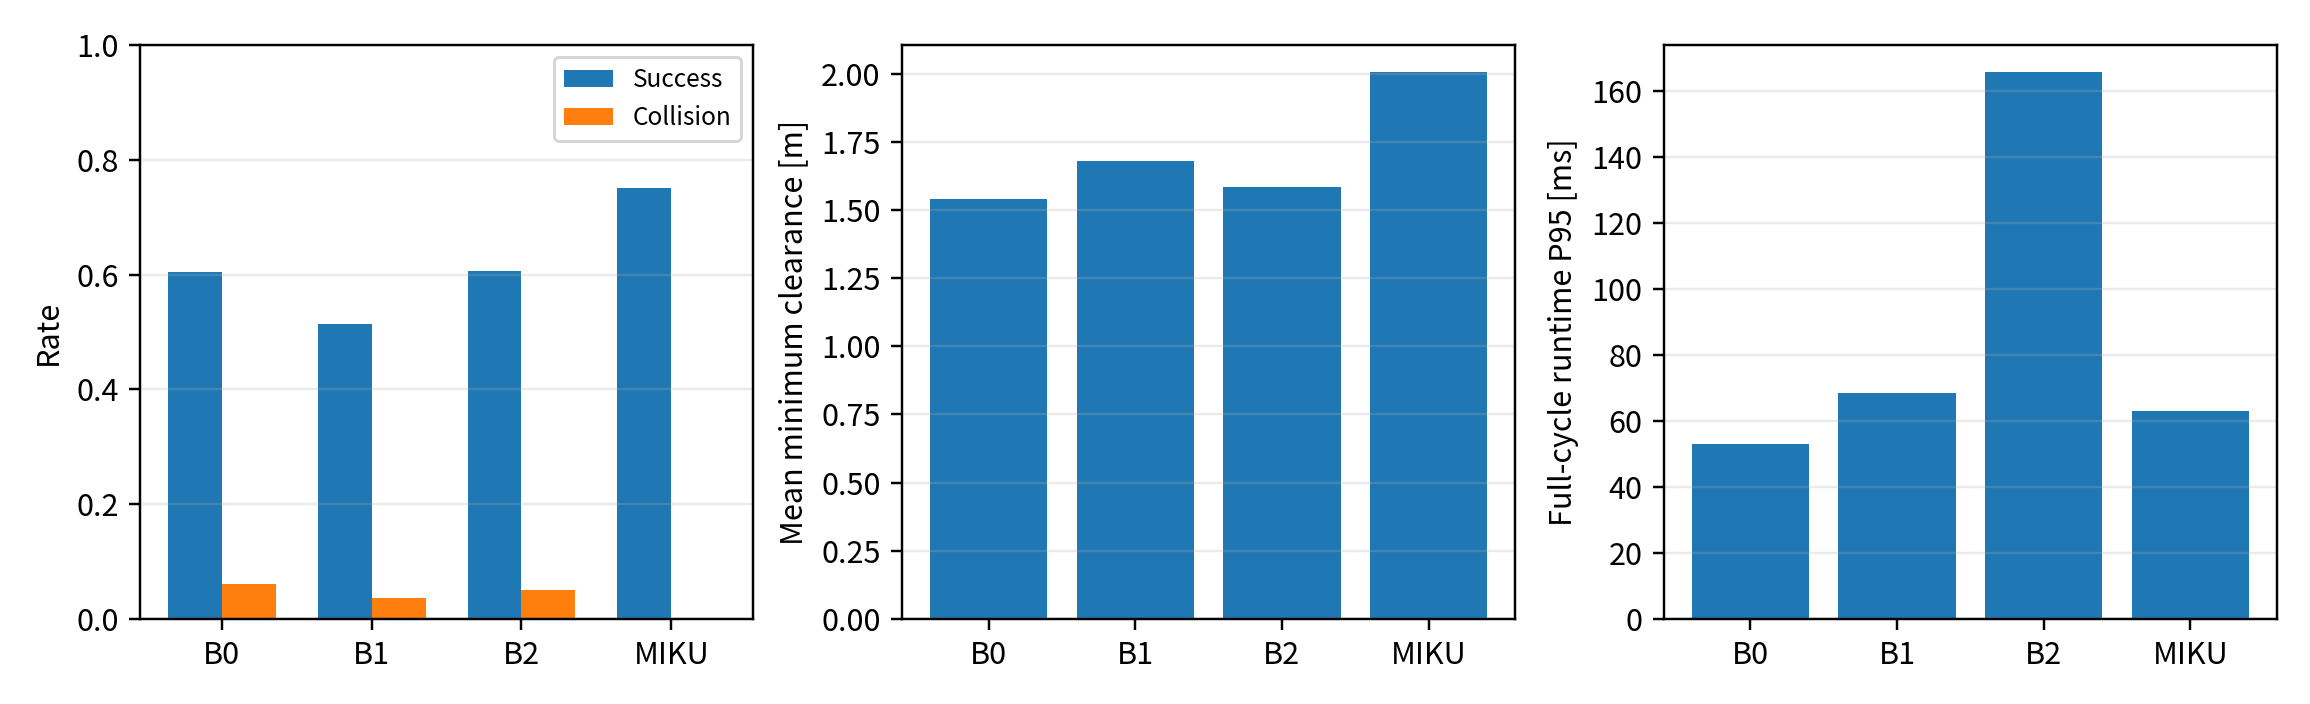
\includegraphics[width=0.96\textwidth]{generated/randomized_summary.png}
\caption{六类配对随机实验的汇总指标}
\label{fig:random_summary}
\end{figure}

\subsection{分场景差异与失效分析}

\begin{table}[htbp]
\centering
\caption{MIKU 与 B0 的分场景无碰撞到达率}
\label{tab:random_by_case}
\small
\begin{tabular}{lrrrr}
\toprule
场景 & B0(\%) & MIKU(\%) & 配对差(百分点) & 95\% CI \\
\midrule
行人横穿 & \RandCrossingBZeroSuccessPct & \RandCrossingMikuSuccessPct & \RandCrossingMikuVsBZeroSuccessDiff & [\RandCrossingMikuVsBZeroSuccessCiLow,\RandCrossingMikuVsBZeroSuccessCiHigh] \\
车辆切入 & \RandCutInBZeroSuccessPct & \RandCutInMikuSuccessPct & \RandCutInMikuVsBZeroSuccessDiff & [\RandCutInMikuVsBZeroSuccessCiLow,\RandCutInMikuVsBZeroSuccessCiHigh] \\
停车+对向车 & \RandParkedBZeroSuccessPct & \RandParkedMikuSuccessPct & \RandParkedMikuVsBZeroSuccessDiff & [\RandParkedMikuVsBZeroSuccessCiLow,\RandParkedMikuVsBZeroSuccessCiHigh] \\
窄路多障碍 & \RandNarrowBZeroSuccessPct & \RandNarrowMikuSuccessPct & \RandNarrowMikuVsBZeroSuccessDiff & [\RandNarrowMikuVsBZeroSuccessCiLow,\RandNarrowMikuVsBZeroSuccessCiHigh] \\
多动态交织 & \RandInterleavedBZeroSuccessPct & \RandInterleavedMikuSuccessPct & \RandInterleavedMikuVsBZeroSuccessDiff & [\RandInterleavedMikuVsBZeroSuccessCiLow,\RandInterleavedMikuVsBZeroSuccessCiHigh] \\
预测含噪 & \RandNoiseBZeroSuccessPct & \RandNoiseMikuSuccessPct & \RandNoiseMikuVsBZeroSuccessDiff & [\RandNoiseMikuVsBZeroSuccessCiLow,\RandNoiseMikuVsBZeroSuccessCiHigh] \\
\bottomrule
\end{tabular}
\end{table}

表~\ref{tab:random_by_case}显示汇总差异由窄路多障碍类驱动：该类中 MIKU 比 B0 高 \RandNarrowMikuVsBZeroSuccessDiff 个百分点，95\% CI [\RandNarrowMikuVsBZeroSuccessCiLow,\RandNarrowMikuVsBZeroSuccessCiHigh]。这与差异化裕度避免小尺寸锥桶与边界重复挤占通道的机制一致。相反，行人横穿与多动态交织类的配对差分别为 \RandCrossingMikuVsBZeroSuccessDiff 和 \RandInterleavedMikuVsBZeroSuccessDiff 个百分点，说明单次到达时间查询可在动态交织中选到不利的横向同伦类。这是方法的适用边界，而不是可通过汇总平均隐去的离群值。

含噪类中 MIKU 的无碰撞到达率为 \RandNoiseMikuSuccessPct\%，碰撞率为 \RandNoiseMikuCollisionPct\%，均明显差于无噪的车辆切入类。失败清单逐例保留种子、方法、进度比与最小间距；主要失效是时域内未到达/降级停车，而含噪类还暴露出预测偏差下安全裕度不足。

\subsection{联合参照与滚动重规划补充实验}

B3-JointReference 在 $(t,s,l,v,\dot l)$ 上同步搜索，公开网格分辨率依次为 0.5\,s、0.5\,m、0.25\,m、1.0\,m/s 与 0.5\,m/s，每层确定性保留至多 20,000 个状态。该方法与 MIKU 共享车辆实体尺寸、道路边界、纵向加减速和横向运动上限，但不使用顺序路径/速度 QP。由于它含 beam 截断且网格离散，只作为质量--开销参照，不称为连续全局最优。

\begin{table}[htbp]
\centering
\caption{小规模联合参照与滚动重规划补充结果}
\label{tab:supplementary_protocols}
\small
\begin{tabular}{llrrrr}
\toprule
协议 & 方法 & $n$ & 到达率(\%) & 碰撞率(\%) & P95耗时(ms) \\
\midrule
联合网格子集 & B3 & \JointCaseCount & \JointBThreeSuccessPct & \JointBThreeCollisionPct & \JointBThreeRuntimePninetyfive \\
联合网格子集 & MIKU & \JointCaseCount & \JointMikuSuccessPct & \JointMikuCollisionPct & \JointMikuRuntimePninetyfive \\
滚动重规划子集 & B0 & \ClosedCaseCount & \ClosedBZeroSuccessPct & \ClosedBZeroCollisionPct & \ClosedBZeroRuntimePninetyfive \\
滚动重规划子集 & MIKU & \ClosedCaseCount & \ClosedMikuSuccessPct & \ClosedMikuCollisionPct & \ClosedMikuRuntimePninetyfive \\
\bottomrule
\end{tabular}
\end{table}

在每类 5 个种子的 \JointCaseCount 个配对子集中，B3 与 MIKU 的无碰撞到达率分别为 \JointBThreeSuccessPct\% 和 \JointMikuSuccessPct\%，配对差为 \JointMikuVsBThreeSuccessDiff 个百分点（95\% CI [\JointMikuVsBThreeSuccessCiLow,\JointMikuVsBThreeSuccessCiHigh]）。B3 单独成功的配对有 \JointBThreeOnlySuccessCount 个，MIKU 单独成功的配对有 \JointMikuOnlySuccessCount 个；这些不一致个例提示顺序解耦可能遗漏联合搜索找到的轨迹，但由于两者保护带定义不同，不能把差异全部归因于解耦结构；跨零的置信区间也不支持总体差异声称。B3 的真值碰撞率为 \JointBThreeCollisionPct\%，MIKU 为 \JointMikuCollisionPct\%；B3 的 P95 完整搜索耗时为 \JointBThreeRuntimePninetyfive\,ms，MIKU 为 \JointMikuRuntimePninetyfive\,ms。粗网格和 0.10\,m 固定保护带不足以抵御含噪输入；B3 只是质量--开销参照，不是安全上界或连续全局最优解。

滚动实验对每类 10 个种子执行“规划 0.5\,s、更新自车与障碍物、再规划”，共 \ClosedCaseCount 个配对场景。MIKU 与 B0 的到达率分别为 \ClosedMikuSuccessPct\% 和 \ClosedBZeroSuccessPct\%，配对差为 \ClosedMikuVsBZeroSuccessDiff 个百分点（95\% CI [\ClosedMikuVsBZeroSuccessCiLow,\ClosedMikuVsBZeroSuccessCiHigh]）。两者碰撞率分别为 \ClosedMikuCollisionPct\% 和 \ClosedBZeroCollisionPct\%，差值为 \ClosedMikuVsBZeroCollisionDiff 个百分点（95\% CI [\ClosedMikuVsBZeroCollisionCiLow,\ClosedMikuVsBZeroCollisionCiHigh]），因而小样本到达率改善不能被解读为安全性改善。这里的耗时是单场景全部规划周期的累计墙钟时间；固定运行顺序和小样本使其只用于规模描述。总体到达率偏低，表明 0.5\,s 执行步长与有限场景时域下仍有大量停车/未到达，不能据此声称完整闭环性能成熟。

\subsection{消融决策与限制}

确定性机理消融显示，差异化裕度是窄路压力构型的活跃组件；关闭分组与最大间隙使密集施工的手工临界构型失败。但对该构型施加很小的几何扰动后，组级改善未保持，因而本文只把它作为机理证据。前缀最大间隙的精确性与该性能鲁棒性是两个不同命题：前者已由定理和 4,000 例穷举 oracle 支持，后者仍受场景分布与上游边界误差影响。

经修正的占用补集安全时窗能表达先通过和后通过，也通过了随机点集 oracle；但开启它后没有在当前压力场景中形成独立正收益，并在动静混合场景出现可重复回归。按预先规定的决策门，它已从主方法关闭，不作为性能贡献。

\subsection{灵敏度分析}

在 P1--P4 中每个场景对 5 个威胁度权重同时施加 $\pm\SensPerturbPct\%$ 均匀扰动并重新归一，每场景 100 次的安全裕度最大相对变化为 \SensWorstRelDev\%。另对每场景 \SensTrajectoryTrialCount 组权重扰动重新运行完整规划，80 条轨迹均到达终点，相对基准的最大横向偏移变化为 \SensOneTrajectoryMaxLateralDev\,m，终点进度和 jerk RMS 在报告精度下未变。这只支持权重局部稳定性：对 $\tau(s)$ 施加 $\pm20\%$、动态障碍物纵向速度施加 $\pm0.5$\,m/s、横向位置施加 $\pm0.2$\,m 的 \SensSingleFactorCount 个对称端点中，到达率仅为 \SensSingleFactorSuccessPct\%；两个动态压力场景的 \SensDynamicSingleFactorCount 个端点中仅为 \SensDynamicSingleFactorSuccessPct\%。因此方法对权重的局部稳定不能外推为对时序与预测误差的鲁棒性。

主实验是有限时域规划轨迹对真值预测的配对回放；补充滚动实验闭合了规划器状态更新，但仍不是实车路测，也未覆盖感知器、控制器与车辆执行器构成的系统闭环。B3 仅有 30 例且采用粗网格与 beam 截断。因此，这些数据只支持本文明示的随机生成分布与 Apollo 规划器在环结论，不支持对自然交通分布或实车安全性的外推。

% ====== 5 结论 ======
\section{结论}
\label{sec:conclusion}

本文将道路、自车尺寸与障碍物裕度统一到自车中心语义，并证明多障碍物最大间隙只需考察排序后的 $k+1$ 个连续分割。前缀最大扫描把单截面求解降为 $O(k\log k)$，4,000 个固定种子实例与穷举 oracle 一致。在 \RandCaseCount 个配对随机实例中，MIKU 相对 B0 的无碰撞到达率汇总差值为 \RandAllMikuVsBZeroSuccessDiff 个百分点，95\% CI [\RandAllMikuVsBZeroSuccessCiLow,\RandAllMikuVsBZeroSuccessCiHigh]；但碰撞率没有降低，且改善集中在窄路分布。

横穿行人与多动态交织类的负差值表明，一次到达时间查询不能代替联合时空协调。30 例联合参照中，B3 单独到达的配对有 \JointBThreeOnlySuccessCount 个，MIKU 单独到达的配对有 \JointMikuOnlySuccessCount 个；到达率差的 95\% CI [\JointMikuVsBThreeSuccessCiLow,\JointMikuVsBThreeSuccessCiHigh] 跨零，而且两者保护带定义不同，因而这些个例只提示可行性差异，不能证明联合方法的总体优势或将差异全部归因于解耦结构。60 例规划器滚动重规划子集中，MIKU 相对 B0 的到达率差为 \ClosedMikuVsBZeroSuccessDiff 个百分点，但总体到达率只有 \ClosedMikuSuccessPct\%，且 MIKU 出现 \ClosedMikuCollisionPct\% 的碰撞率。经修正的速度侧安全时窗因无独立正收益已从主方法剔除。后续工作需要扩展联合参照与滚动样本，并加入感知、控制器和执行器的软硬件在环实验；在此之前，本文结论只适用于已公开的随机生成分布和 Apollo 规划器环境。

\printbibliography[heading=bibintoc,title={参考文献}]

\end{document}
